% !Mode:: "TeX:UTF-8"

\documentclass[openany,twoside,nofonts,AutoFakeBold,UTF8]{ctexbook}
\usepackage{blindtext}
\usepackage{scrextend}
\usepackage{nomencl}
\usepackage{blkarray}
\usepackage{makecell}
\usepackage{wrapfig}
\usepackage{bbm}
\usepackage{amsmath}
% \addtokomafont{labelinglabel}{\sffamily}
\renewcommand{\footnotesize}{\fontsize{9pt}{10pt}\selectfont}
\def\bd{\boldsymbol}        % 加粗(向量) boldsymbol
\def\e{\mathrm{e}}          % Euler's number
\def\add{\vspace{1ex}}      % 增加行间距
\def\del{\vspace{-1.5ex}}   % 减少行间距
\DeclareMathOperator*{\argmax}{arg\,max}  % 定义取最大值的参数 \argmax_{}

% !Mode:: "TeX:UTF-8"

\usepackage[a4paper,top=21.5mm,bottom=19.5mm,left=26mm,right=26mm,includehead,includefoot]{geometry}					% 控制页面尺寸
\usepackage{titletoc}       % 控制目录的宏包
\usepackage{titlesec}       % 控制标题的宏包
\usepackage{fancyhdr}       % 页眉和页脚的相关定义
\usepackage{color}          % 支持彩色
\usepackage{graphicx}		% 处理图片
\usepackage{tabularx}		% 可伸缩表格
\usepackage{multirow}       % 表格可以合并多个row
\usepackage{booktabs}       % 表格横的粗线;\specialrule{1pt}{0pt}{0pt}
\usepackage{longtable}      % 支持跨页的表格。
\usepackage{enumitem}       % 使用enumitem宏包,改变列表项的格式
\usepackage{amsmath}        % 公式宏包
\usepackage{amssymb}		% 符号宏包
\usepackage{bm}				% 处理数学公式中的黑斜体的宏包
\usepackage{lmodern}		% 数学公式字体
\usepackage[amsmath,thmmarks,hyperref]{ntheorem}	% 定理类环境宏包
\usepackage[hang]{subfigure}						% 图形或表格并排排列
\usepackage[subfigure]{ccaption}					% 支持双语标题
\usepackage[sort&compress,numbers]{natbib}			% 支持引用缩写的宏包
\usepackage{fontspec}		% 字体设置宏包
%\usepackage{etoolbox}		% primarily towards LaTeX class and package authors.
%\usepackage{xltxtra}		% 提供了针对XeTeX的改进,自动调用xunicode宏包

% 生成有书签的 pdf 及其开关, 该宏包应放在所有宏包的最后, 宏包之间有冲突
\usepackage[xetex,
            bookmarksnumbered=true,
            bookmarksopen=true,
            colorlinks=false,
            pdfborder={0 0 1},
            citecolor=blue,
            linkcolor=red,
            anchorcolor=green,
            urlcolor=blue,
            breaklinks=true
            ]{hyperref}

% 算法的宏包,注意宏包兼容性,先后顺序为float、hyperref、algorithm(2e),否则无法生成算法列表
\usepackage[plainruled,linesnumbered,algochapter]{algorithm2e}
% \usepackage[linesnumbered,ruled,vlined]{algorithm2e}
\SetKwInput{KwIn}{输入}  %<---细节与重点
\SetKwInput{KwOut}{输出}  %<---细节与重点

% \usepackage{listings}		% 为了避免与页眉的兼容问题可将listings放入table环境中
% \definecolor{codegreen}{rgb}{0,0.6,0}
% \definecolor{codepurple}{rgb}{0.58,0,0.82}
% \lstset{%
% 	language={[ISO]C++},				% 设置语言
% 	alsolanguage=Matlab,				% 可以添加多个语言选项
% 	alsolanguage=Verilog,
% 	morekeywords={numerictype,fimath,fipref,fi,trh},
% 	commentstyle=\color{codegreen},		% 注释颜色
% 	keywordstyle=\color{blue},			% 代码关键字颜色
% 	stringstyle=\color{codepurple},		% 代码中字符串颜色
% 	frame=single,			% 设置边框, 
% 	xleftmargin=1.7em,		% 设定listing左边空白 
% 	numbers=left,			% 左侧显示行号
% 	numberstyle=\small,		% 行号字体用小号
% 	breaklines=true,		% 对过长的代码自动换行 
% 	columns=flexible,		% 调整字符之间的距离
% 	tabsize=4				% table 长度
% }
%%%% 设置代码块 %%%%
% 在vscode中使用minted需要先配置python解释器, Ctrl+Shift+P, 输入Python: Select Interpreter选择安装了Pygments的Python版本. 再在setting.json中xelatex和pdflatex的参数中加入 "--shell-escape", 即可
% TeXworks中配置方法参考: https://blog.csdn.net/RobertChenGuangzhi/article/details/108140093
\usepackage{minted}
\renewcommand{\theFancyVerbLine}{
    \sffamily\textcolor[rgb]{0.5,0.5,0.5}{\scriptsize\arabic{FancyVerbLine}}} % 修改代码前序号大小
% 加入不同语言的代码块
\newmintinline{cpp}{fontsize=\small, linenos, breaklines, frame=lines}
\newminted{cpp}{fontsize=\small, baselinestretch=1, linenos, breaklines, frame=lines}
\newmintedfile{cpp}{fontsize=\small, baselinestretch=1, linenos, breaklines, frame=lines}
\newmintinline{matlab}{fontsize=\small, linenos, breaklines, frame=lines}
\newminted{matlab}{fontsize=\small, baselinestretch=1, mathescape, linenos, breaklines, frame=lines}
\newmintedfile{matlab}{fontsize=\small, baselinestretch=1, linenos, breaklines, frame=lines}
\newmintinline{python}{fontsize=\small, linenos, breaklines, frame=lines, python3}  % 使用\pythoninline{代码}
\newminted{python}{fontsize=\small, baselinestretch=1, linenos, breaklines, frame=lines, python3}  % 使用\begin{pythoncode}代码\end{pythoncode}
\newmintedfile{python}{fontsize=\small, baselinestretch=1, linenos, breaklines, frame=lines, python3}  % 使用\pythonfile{代码地址}

% 带圆圈的脚注
\usepackage{pifont}
\usepackage[flushmargin,para,symbol*]{footmisc}
\DefineFNsymbols{circled}{{\ding{192}}{\ding{193}}{\ding{194}}
	{\ding{195}}{\ding{196}}{\ding{197}}{\ding{198}}{\ding{199}}{\ding{200}}{\ding{201}}}
\setfnsymbol{circled}

% 字体设置,Windows自带黑体(simhei.ttf)和宋体(simsun.ttf)
\defaultfontfeatures{Mapping=tex-text}
\setmainfont{Times New Roman}
% \setsansfont{Arial}
\setCJKmainfont{SimSun}
\setCJKsansfont{SimHei}
\setCJKfamilyfont{hei}{SimHei}
\newcommand{\hei}{\CJKfamily{hei}}

% 外文文献pdf插入
\usepackage{pdfpages}

% 符号表
\graphicspath{{figures/}}

%===================================== Cover and TOC =====================================
\begin{document}
% !Mode:: "TeX:UTF-8" 

% 备注
\long\def\zhao#1{\textcolor{red}{\bf **#1**}}

%========================================= Font ==========================================
% 定义字号
\newcommand{\yihao}{\fontsize{26pt}{26pt}\selectfont}       % 一号, 1.倍行距
\newcommand{\xiaoyi}{\fontsize{24pt}{24pt}\selectfont}      % 小一, 1.倍行距
\newcommand{\erhao}{\fontsize{22pt}{22pt}\selectfont}		% 二号, 1.倍行距
\newcommand{\xiaoer}{\fontsize{18pt}{18pt}\selectfont}      % 小二, 单倍行距
\newcommand{\sanhao}{\fontsize{16pt}{16pt}\selectfont}      % 三号, 1.倍行距
\newcommand{\xiaosan}{\fontsize{15pt}{15pt}\selectfont}     % 小三, 1.倍行距
\newcommand{\sihao}{\fontsize{14pt}{14pt}\selectfont}       % 四号, 1.倍行距
\newcommand{\xiaosi}{\fontsize{12pt}{12pt}\selectfont}      % 小四, 1.倍行距
\newcommand{\wuhao}{\fontsize{10.5pt}{10.5pt}\selectfont}   % 五号, 单倍行距
\newcommand{\xiaowu}{\fontsize{9pt}{9pt}\selectfont}        % 小五, 单倍行距

% 默认字体
\makeatletter
\renewcommand\normalsize{%
	\@setfontsize\normalsize{12pt}{12pt}%
	\setlength\abovedisplayskip{8pt}%
	\setlength\abovedisplayshortskip{8pt}%
	\setlength\belowdisplayskip{\abovedisplayskip}%
	\setlength\belowdisplayshortskip{\abovedisplayshortskip}%
	\let\@listi\@listI%
}

% 设置行距和段落间垂直距离
\setlength{\parindent}{2em}
\setlength{\parskip}{3pt plus1pt minus1pt}
\def\defaultfont{\renewcommand{\baselinestretch}{1.5}\normalsize\selectfont}

% 设置字间距,使每行37个字,若要减少每行字数(一般以34个),将0.56pt的值增加
\renewcommand{\CJKglue}{\hskip 0.56pt plus 0.08\baselineskip}

% 公式跨页设置,公式之前可以换页,公式出现在页面顶部
\predisplaypenalty=0
\allowdisplaybreaks[4]

%========================================= TOC ===========================================
% 中文目录格式定义
\renewcommand\contentsname{目\quad 录}
\titlecontents{chapter}[3.8em]{\hspace{-3.8em}}{\thecontentslabel~~}{}{\titlerule*[4pt]{.}\contentspage}
\dottedcontents{section}[38pt]{}{22pt}{0.3pc}
\dottedcontents{subsection}[70pt]{}{32pt}{0.3pc}

% 英文目录格式定义: 细点\@dottedtocline  粗点\@dottedtoclinebold
\renewcommand*\l@chapter{\@dottedtocline{0}{0em}{5em}}
\renewcommand*\l@section{\@dottedtocline{1}{1em}{1.8em}}
\renewcommand*\l@subsection{\@dottedtocline{2}{2.9em}{2.5em}}
\def\@dotsep{0.75}           % 定义英文目录的点间距
\setlength\leftmargini {50pt}
\setlength\leftmarginii {50pt}
\def\engcontentsname{CONTENTS}
\newcommand\tableofengcontents{
	\@restonecolfalse
	\chapter*{\engcontentsname  %chapter*上移一行,避免在toc中出现。
		\@mkboth{%
			\engcontentsname}{\engcontentsname}}
	\@starttoc{toe}%
	\if@restonecol\twocolumn\fi
}

%======================================= Chapter =========================================
% 章节格式定义
\CTEXsetup[number={\arabic{chapter}}]{chapter}
\renewcommand\chaptername{\thechapter}
\CTEXsetup[name={,}]{chapter}
\setcounter{secnumdepth}{4} \setcounter{tocdepth}{2}
\titleformat{\chapter}{\center\sanhao}{\chaptertitlename}{0.5em}{}
\titlespacing{\chapter}{0pt}{-5mm}{5mm}
\titleformat{\section}{\xiaosan}{\thesection}{0.5em}{}
\titlespacing{\section}{0pt}{3mm}{3mm}
\titleformat{\subsection}{\sihao}{\thesubsection}{0.5em}{}
\titlespacing{\subsection}{2.13em}{3mm}{3mm}

% 重新定义BiChapter命令,可实现标题手动换行,但不影响目录
\def\BiChapter{\relax\@ifnextchar [{\@BiChapter}{\@@BiChapter}}
\def\@BiChapter[#1]#2#3{\chapter[#1]{#2}
    \addcontentsline{toe}{chapter}{\xiaosi \thechapter\hspace{0.5em} #3}}
\def\@@BiChapter#1#2{\chapter{#1}
    \addcontentsline{toe}{chapter}{\xiaosi \thechapter\hspace{0.5em}{\boldmath #2}}}
% 定义双标题
\newcommand{\BiSection}[2]{
	\section{#1}
	\addcontentsline{toe}{section}{\protect\numberline{\csname thesection\endcsname}#2}
}
\newcommand{\BiSubsection}[2]{
	\subsection{#1}
	\addcontentsline{toe}{subsection}{\protect\numberline{\csname thesubsection\endcsname}#2}
}
\newcommand{\BiSubsubsection}[2]{
    \subsubsection{#1}
    \addcontentsline{toe}{subsubsection}{\protect\numberline{\csname thesubsubsection\endcsname}#2}
}

% 该附录命令适用于有章节的完整附录和用于发表文章和简历的附录
\newcommand{\BiAppChapter}[2]{
	\phantomsection 
	\chapter{#1}
	\addcontentsline{toe}{chapter}{\xiaosi Appendix \thechapter~~#2}
}
\newcommand{\BiAppendixChapter}[2]{
	\phantomsection
	\markboth{#1}{#1}
	\addcontentsline{toc}{chapter}{\xiaosi #1}
	\addcontentsline{toe}{chapter}{\xiaosi #2}  \chapter*{#1}
}
\newcommand{\Abstract}[2]{
	\phantomsection
	\markboth{#1}{#1}
	\chapter*{#1}
}


%======================================== Header =========================================
% 定义页眉和页脚
\newcommand{\makeheadrule}{
\rule[8pt]{\textwidth}{0.4pt} \\[-22pt]
\rule{\textwidth}{0.4pt}}
\renewcommand{\headrule}{
    {\if@fancyplain\let\headrulewidth\plainheadrulewidth\fi
     \makeheadrule}}
\pagestyle{fancyplain}

% 不要注销这一行,否则页眉会变成:“第1章1  绪论”样式
\renewcommand{\chaptermark}[1]{\markboth{\chaptertitlename~\ #1}{}}
\fancyhf{}
\fancyhead[CO]{\wuhao\leftmark}
\fancyhead[CE]{\wuhao 西安交通大学本科毕业设计(论文)}%
\fancyfoot[LE,RO]{\wuhao\thepage}

%======================================= Theorem =========================================
% 定理环境格式定义
\theoremstyle{plain}
\theorembodyfont{\rmfamily}
\theoremheaderfont{\hei\rmfamily}
\setlength{\theorempreskipamount}{8pt}
\setlength{\theorempostskipamount}{8pt}
\theoremseparator{:}
\theoremsymbol{$\Diamond$} \newtheorem{definition}{\hskip 2em \hei 定义}[chapter]
\theoremsymbol{$\blacklozenge$} \newtheorem{example}{\hskip 2em \hei 例}[chapter]
\theoremsymbol{$\square$} \newtheorem{theorem}{\hskip 2em \hei 定理}[chapter]
\theoremsymbol{$\blacksquare$} \newtheorem*{proof}{\hskip 2em \hei 证明}

%========================================= FTE ===========================================
% 图表公式的编号为1-1格式,子图编号为 a) 的格式
\renewcommand{\thefigure}{\arabic{chapter}-\arabic{figure}}
\renewcommand{\thesubfigure}{(\alph{subfigure})}
\renewcommand{\p@subfigure}{\thefigure~}
\renewcommand{\thetable}{\arabic{chapter}-\arabic{table}}%使表编号为 7-1 的格式
\renewcommand{\theequation}{\arabic{chapter}-\arabic{equation}}%使公式编号为 7-1 的格式

% 定制浮动图形和表格标题样式
\captionnamefont{\wuhao}
\captiontitlefont{\wuhao}
\captiondelim{~~}
\hangcaption
\renewcommand{\subcapsize}{\wuhao}
% \setlength{\abovecaptionskip}{0pt}
\setlength{\abovecaptionskip}{-4ex}  % 由于minted会增大图像与标题间距需要进行缩小
\setlength{\belowcaptionskip}{0pt}

% 关于公式的几个定义
\renewcommand{\Re}{\mathrm{Re}}
\renewcommand{\Im}{\mathrm{Im}}
\newcommand{\mbf}[1]{\mathbf{#1}}
\newcommand{\Exp}{\mathrm{E}}
\newcommand{\dif}{\mathrm{d}}
\newcommand{\seq}[2]{#1_1,#1_2,\cdots,#1_#2}
\newcommand{\iprod}[2]{\langle #1,#2 \rangle}

% 调整罗列环境的布局
\setitemize{leftmargin=3.23em,itemsep=0em,partopsep=0em,parsep=0em,topsep=-0em}
% \setenumerate{leftmargin=3.45em,itemsep=0em,partopsep=0em,parsep=0em,topsep=0em}
\setenumerate{leftmargin=2em,itemsep=0em,partopsep=0em,parsep=0em,topsep=0em}

% 自定义项目列表标签及格式 \begin{publist} 列表项 \end{publist}
\newcounter{pubctr} %自定义新计数器
\newenvironment{publist}{
	\begin{list}{[\arabic{pubctr}]}{
     \usecounter{pubctr}
     \setlength{\leftmargin}{2em}     % 左边界
     \setlength{\labelsep}{1em}       % 标号和列表项之间的距离,默认0.5em
     \setlength{\parsep}{0ex}         % 段落间距
     \setlength{\itemsep}{0ex}        % 标签间距
    }}
{\end{list}}%

% 更改算法标题
\renewcommand{\algorithmcfname}{算法}
\renewcommand{\algocf@captiontext}[2]{\wuhao#1\algocf@typo ~ \AlCapFnt{}#2}
\renewcommand\thealgocf{\csname the\algocf@within\endcsname-\@arabic\c@algocf}
\SetAlCapSty{textrm}
\SetAlCapSkip{1ex}

% 更改代码标题
% \renewcommand{\lstlistingname}{代码}
% \renewcommand{\thelstlisting}{\arabic{chapter}-\arabic{lstlisting}}

%======================================== Other ==========================================
% 避免宏包 hyperref 和 arydshln 不兼容带来的目录链接失效的问题。
\def\temp{\relax}
\let\temp\addcontentsline
\gdef\addcontentsline{\phantomsection\temp}
\gdef\hitempty{}

\renewcommand\frontmatter{\cleardoublepage
	\@mainmatterfalse
	\pagenumbering{Roman}
}

% 引用改为上标
\newcommand{\upcite}[1]{\textsuperscript{\cite{#1}}}

\makeatother

\begin{center}\Large
通过计算机视觉及离线强化学习游玩非嵌入式卡牌类即时战略游戏
\end{center}
%%% 摘要 %%%
\section{摘要}
人工智能在游戏中的研究已经取得了很大的进展,例如棋盘游戏、MOBA游戏、RTS游戏。
然而目前复杂的智能体均为嵌入式开发,即智能体可以直接从游戏底层获取状态信息,与人类玩家所获取的图像信息完全不同,
图像信息中往往带有很多噪声,而这些可能干扰玩家决策,这导致了竞技的不公平性产生,因此复杂的非嵌入式智能体开发仍然是一个挑战。
此外,卡牌类RTS游戏具有复杂的卡牌特征与巨大的状态空间等难点,仍然缺乏解决方案。
我们提出了一种基于非嵌入式离线强化学习的训练策略,通过图像信息输入在即时策略游戏皇室战争(Clash Royale)
\footnote{Clash Roayle是Supcell在芬兰或其他国家的商标,本文中仍和内容均不应视为Supercell的批准或赞助。}中实现实时的自主博弈对局。
由于当前没有关于该游戏的目标识别数据集,因此我们设计了一种生成式数据集用于训练目标识别模型,
我们结合当前目标识别与光学文本识别的前沿算法对图像信息进行特征提取,并使用离线强化学习算法进行训练,
实现了移动设备上的实时图像获取、感知特征融合、智能体决策及设备控制,能够与对手实时对局,并成功战胜了游戏中的内置AI。
本文的全部代码均已开源 \url{https://github.com/wty-yy/katacr}。

\noindent{\textbf{关键词:}} 目标识别;光学文本识别;离线强化学习

%======================================= Main Body =======================================
%%% 正文 %%%
\section{简介}
即时战略游戏(Real-Time Strategy,RTS)通常具有巨大的状态空间、稀疏奖励、信息不完全和策略多样性等特点,
卡牌类RTS游戏是一种特殊的RTS游戏,两名玩家使用手牌进行实时决策对局。
与一般的卡牌类游戏不同,卡牌类RTS游戏与复杂的卡牌特性有关,
也和卡牌的选择与使用的时机有关,卡牌可以在战场中的不同位置使用,
这产生了巨大的状态空间。玩家无法看到其他玩家的手牌,这产生了不完整的信息。
游戏结果需要到对局结束时才能知道是否胜利,因此游戏中的奖励十分稀疏。
进攻、防守、灵活拉扯、控制节奏等策略使比赛具有很大的不确定性。

自从Mnih等人\cite{DQN}在Atari游戏上成功使用深度强化学习(Deep reinforcement learning, DRL)算法超越人类在该游戏上平均水平后,
研究人员们尝试将DRL算法运用于各种游戏中,例如:棋盘游戏(围棋中Silver等人\cite{AlphaGo}的AlphaGO和Vinyals等人\cite{AlphaStar}的AlphaStar),
MOBA游戏(DOTA2中Berner等人\cite{OpenAIFive}的OpenAI Five),RTS游戏(星际争霸中Vinyals等人\cite{AlphaStar}的AlphaStar)。
值得注意的是,在复杂游戏,例如DOTA2和星际争霸中的智能体均为嵌入式模型,
即智能体可以直接从游戏底层直接获取到准确的状态信息,而这种获取游戏状态的方式与人类完全不同。
人类主要通过图像信息理解游戏状态,但图像信息中通常伴有噪声,这些噪声可能干扰玩家决策,
因此不同的状态获取方式会导致游戏竞技上的不公平性产生。
另一方面,嵌入式智能体能够高效地与环境进行交互,所以可以使用在线强化学习算法训练智能体,
例如Mnih等人\cite{DQN}的Deep Q Network(DQN)算法,Schulman等人\cite{PPO}的Proximal Policy Optimization(PPO)算法。
非嵌入式智能体通常与环境交互速度十分缓慢,这也导致在线训练方法成为一大挑战,
而离线强化学习(Offline reinforcement learning)是解决这一类问题的一种方法,
例如Kumar等人\cite{CQL}的Conservative Q-Learning(CQL),Lili Chen等人\cite{DT}的Decision Transformer(DT)。
这些算法通过学习专家数据集,能够在不和环境进行交互情况下学习策略,并最终与真实环境进行交互验证模型性能。

本文我们只关注一款流行的卡牌类RTS游戏,皇室战争(Clash Royale, CR\footnote{\url{https://clashroyale.com/}})。
具体来说,我们设计了如图\ref{fig-framework}所示的一整套非嵌入式智能体游玩CR的交互流程,
包括与移动设备的交互,对图像特征的感知融合,
% 使用计算机视觉模型对图像信息进行处理后,完成特征提取,作为决策模型智能体的输入,
% 设计一种非嵌入式智能体与环境进行感知与交互。
以及智能体决策模型的控制。
本文通过收集专家数据集,
在这种奖励稀疏,且智能体和环境交互速度缓慢的情况下,
使用离线强化学习算法训练智能体,
虽然智能体在训练中没有与真实环境进行过交互,
但是最终却能成功战胜真实游戏中内置的顶级AI。
\begin{figure}[htbp]
  \centering
  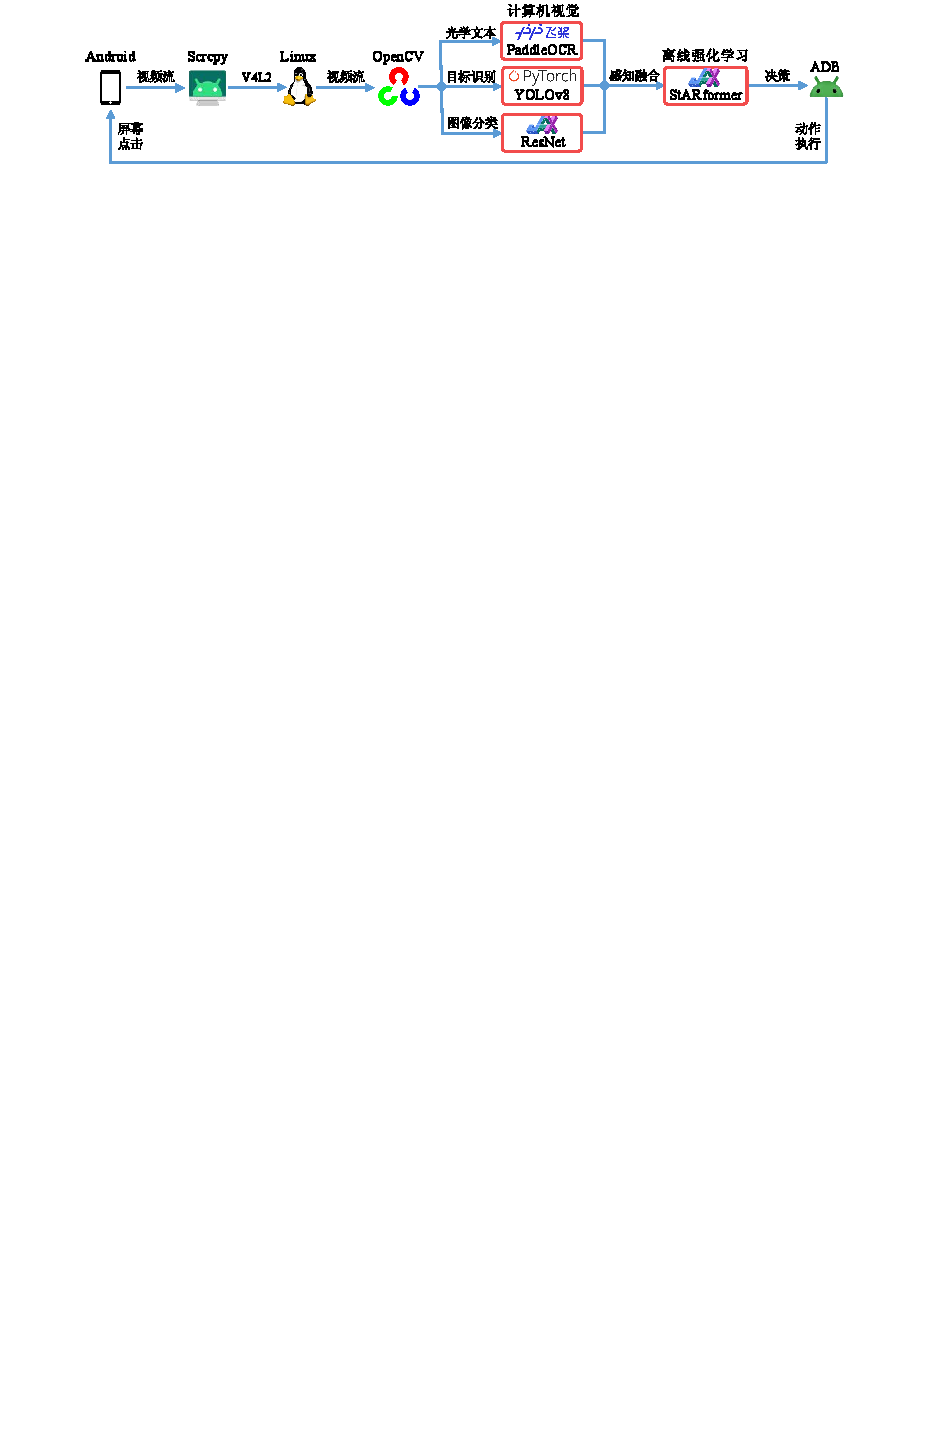
\includegraphics[width=\textwidth]{figures/framework.pdf}
  \caption{Information flow transmission flow chart}\label{fig-framework}
\end{figure}

\section{卡牌即时策略游戏}
皇室战争是一款流行的卡牌类RTS游戏,本文仅考虑经典的一对一对战模式,
双方玩家需要通过实时决策部署手牌来战胜对手,我们测试的游戏版本为2024年5月第59赛季。
\subsection{感知场景}
\begin{figure}[htbp]
  \centering
  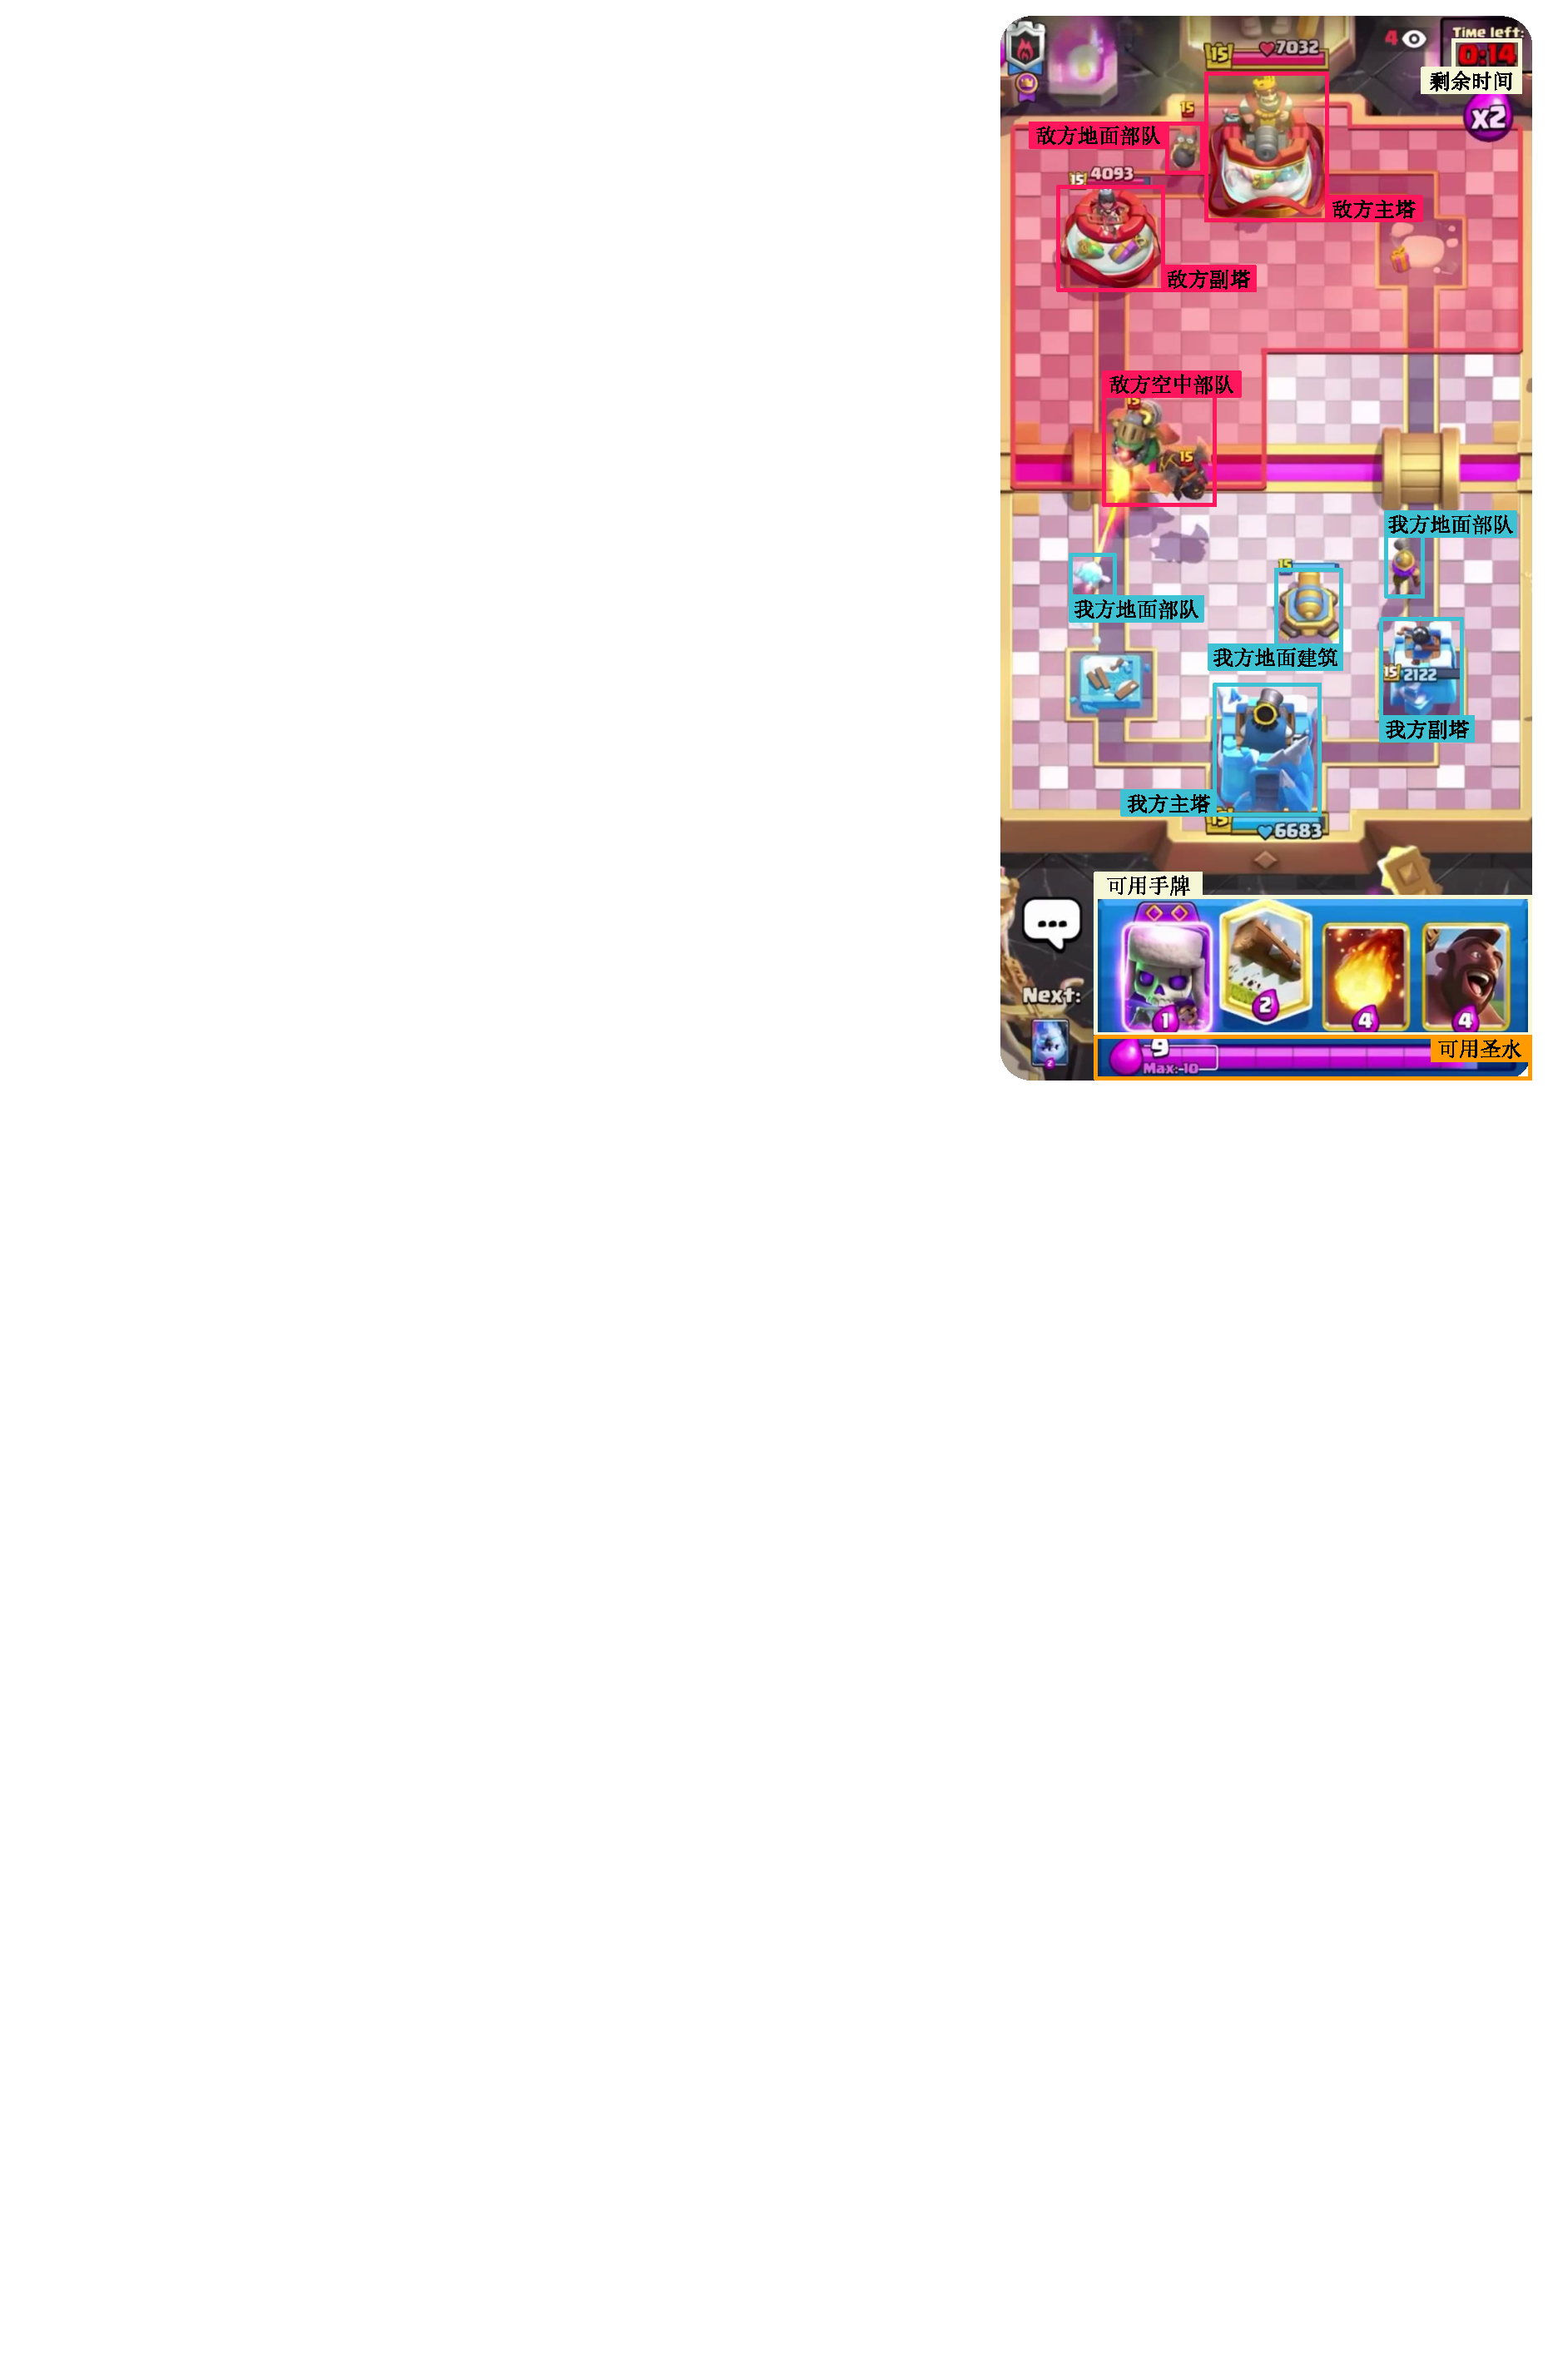
\includegraphics[width=0.5\textwidth]{figures/introduction.pdf}
  \caption{1}\label{fig-introduction}
\end{figure}
在对局过程中,游戏场景如图~\ref{fig-introduction}~所示,
本文所需的感知内容主要分为如下四个主要部分(竞技场,手牌,游戏时间,总圣水)和
竞技场中的三个子部分(主塔,副塔,部队)。

竞技场(Arena)中包括防御塔及双方所部署的部队和建筑物。
竞技场的右上方是当前游戏时间,表示当前阶段所剩的时间。
竞技场的下方是当前手牌和总圣水,手牌包括当前卡牌图像及其所需的圣水费用,
卡牌包含部队、法术、建筑三种,部队分为空中与地面两种。
部队是在竞技场中可移动单位,能够攻击与防御;法术是一种区域效果,
通常可以迅速杀死一群部队;建筑物使用后就被固定在一个位置,攻击在其附近的部队。
总圣水是使用卡牌所需花费的材料,并会随着时间自动回复。

玩家需要在游戏时间内,尽可能多的推掉敌方的防御塔,在下面小结中,
我们将具体介绍游戏的过程,并对游戏状态进行数学建模。
\subsection{游戏过程}
游戏过程包括卡牌轮换和获胜条件两个部分,卡牌轮换是指玩家的手牌在使用后的变换规律,
获胜条件是指在对局结束时判定玩家胜利、平局、失败的条件。
\paragraph{卡牌轮换}
每次对局中双方玩家牌库大小均为8张,在对局开始时,随机在队列中初始化卡牌的出现顺序,
每次从队首取出4张手牌,当玩家使用卡牌后,使用完的卡牌将被重新加入队尾,
所以理论上当一方使用完8张不同卡牌时,可以通过逻辑计算出未出现卡牌类别。
玩家需要基于当前竞技场上的实时状态、手牌类别及总圣水信息,
实时决策卡牌类别的使用位置,采取进攻或防守策略。
\paragraph{获胜条件}\label{win-condition}
每位玩家的目标是摧毁尽可能多的敌方防御塔,优先摧毁敌方主塔的玩家立刻获胜。
游戏中在两种阶段下存在不同的胜利条件:
\begin{enumerate}
  \item 常规时间:持续三分钟,目标为摧毁更多的敌方防御塔,若时间结束时防御塔数量一致,则进入加时赛,
  否则防御塔多的一方获胜。
  \item 加时赛:持续两分钟,在该阶段中,首个摧毁敌方剩余防御塔的玩家获胜,
  若加时赛结束时仍未分出胜负,则比较双方防御塔的最低生命值,最低生命值较高者获胜,若仍未分出胜负,则为平局。
\end{enumerate}
\subsection{游戏状态}\label{sec-game-state}
对于竞技场(Arena)而言,其防御塔、部队的状态由位置、生命值、类别和派别四种参数构成。
\begin{enumerate}
  \item \textbf{位置}~对于第$i$个单位的坐标,将其记为二维离散坐标$\bd{x}_i$,
  表示单位所处于大小$18\times 32$的网格内。
  \item \textbf{类别}~对于第$i$个单位的类别,将其记为一维离散值$c_{i}$,
  这是每个部队或建筑的唯一标签,可选类别范围从$1$到$150$。
  \item \textbf{派别}~对于第$i$个单位的派别,将其记为二值化离散值$bel_{i}$,
  表示单位所从属方(ownship),取值仅在$0$和$1$之中,分别代表我方和敌方单位。
  \item \textbf{生命值}~对于第$i$个单位的生命值,将其记为黑白条状图像$bar_i$,
  在条状图像中记录了每个单位所剩余的生命值。
\end{enumerate}
对于游戏时间,可以通过当前剩余时间换算出经过的总时间$t$,一场对局的总时间不超过$300$秒,
因此时间的取值范围为$0\leqslant t\leqslant 300$。
对于手牌信息,当每次使用手牌后,手牌位为会出现$1$秒的空置时间,当手牌位非空时,
手牌信息由每个位置的手牌类别构成,记为四维离散坐标$\bd{\text{card}}$,
由于每个玩家最多携带$8$张手牌,因此每个维度上数值范围在$1$到$8$之间。
总圣水信息记为一维离散值$\text{elixir}$,由于总圣水上限为$10$,
因此圣水的取值范围为$0\leqslant \text{elixir}\leqslant 10$。

\section{生成式数据集}\label{sec-generation-dataset}
对于图\ref{fig-introduction}竞技场中第$i$个单位$u_i$,
由 \ref{sec-game-state} 中定义,$u_i$可以表示为$(\bd{x}_i, c_i, bel_i,bar_i)$,
本章节关注于如何建立一个生成式数据集包含$\bd{x}_i,c_i,bel_i$信息。

由于训练目标识别模型需要大量带边界框标签的图像,而目前没有任何有关该游戏的目标识别数据集,
如果人工逐帧标记低效且成本高昂,因此我们提出一种高效的带标签图像生成方案,
并在重构后的YOLOv8模型上训练,再在真实视频流数据集验证集中进行验证,
得到了如表\ref{table-yolo}所示的极高准确率,验证了生成式数据集的可行性。

生成式数据集需要基于每个类别单位的切片图像,切片图像与识别模型的更新流程如图\ref{fig-generation-dataset}所示,
其中左上部分的“原视频流”为一个回合的视频数据,若存在之前训练的目标识别模型,则
使用该模型进行对视频流进行辅助标记,从而获得“辅助标记视频流”,再进行手工标记,否则直接对“原视频流”进行手工标记;
在手工标记中,以0.5秒作为标记间隔,进行人工目标框标记;然后将目标框和原图像同时传入到SAM模型当中获取前景分割,
将分割后的结果进行人工筛选获得“切片数据集”;基于已完成的切片数据集,利用生成式数据集算法,对目标识别模型进行迭代更新,
从而用于下一次的辅助标记过程。
\begin{figure}[htbp]
  \centering
  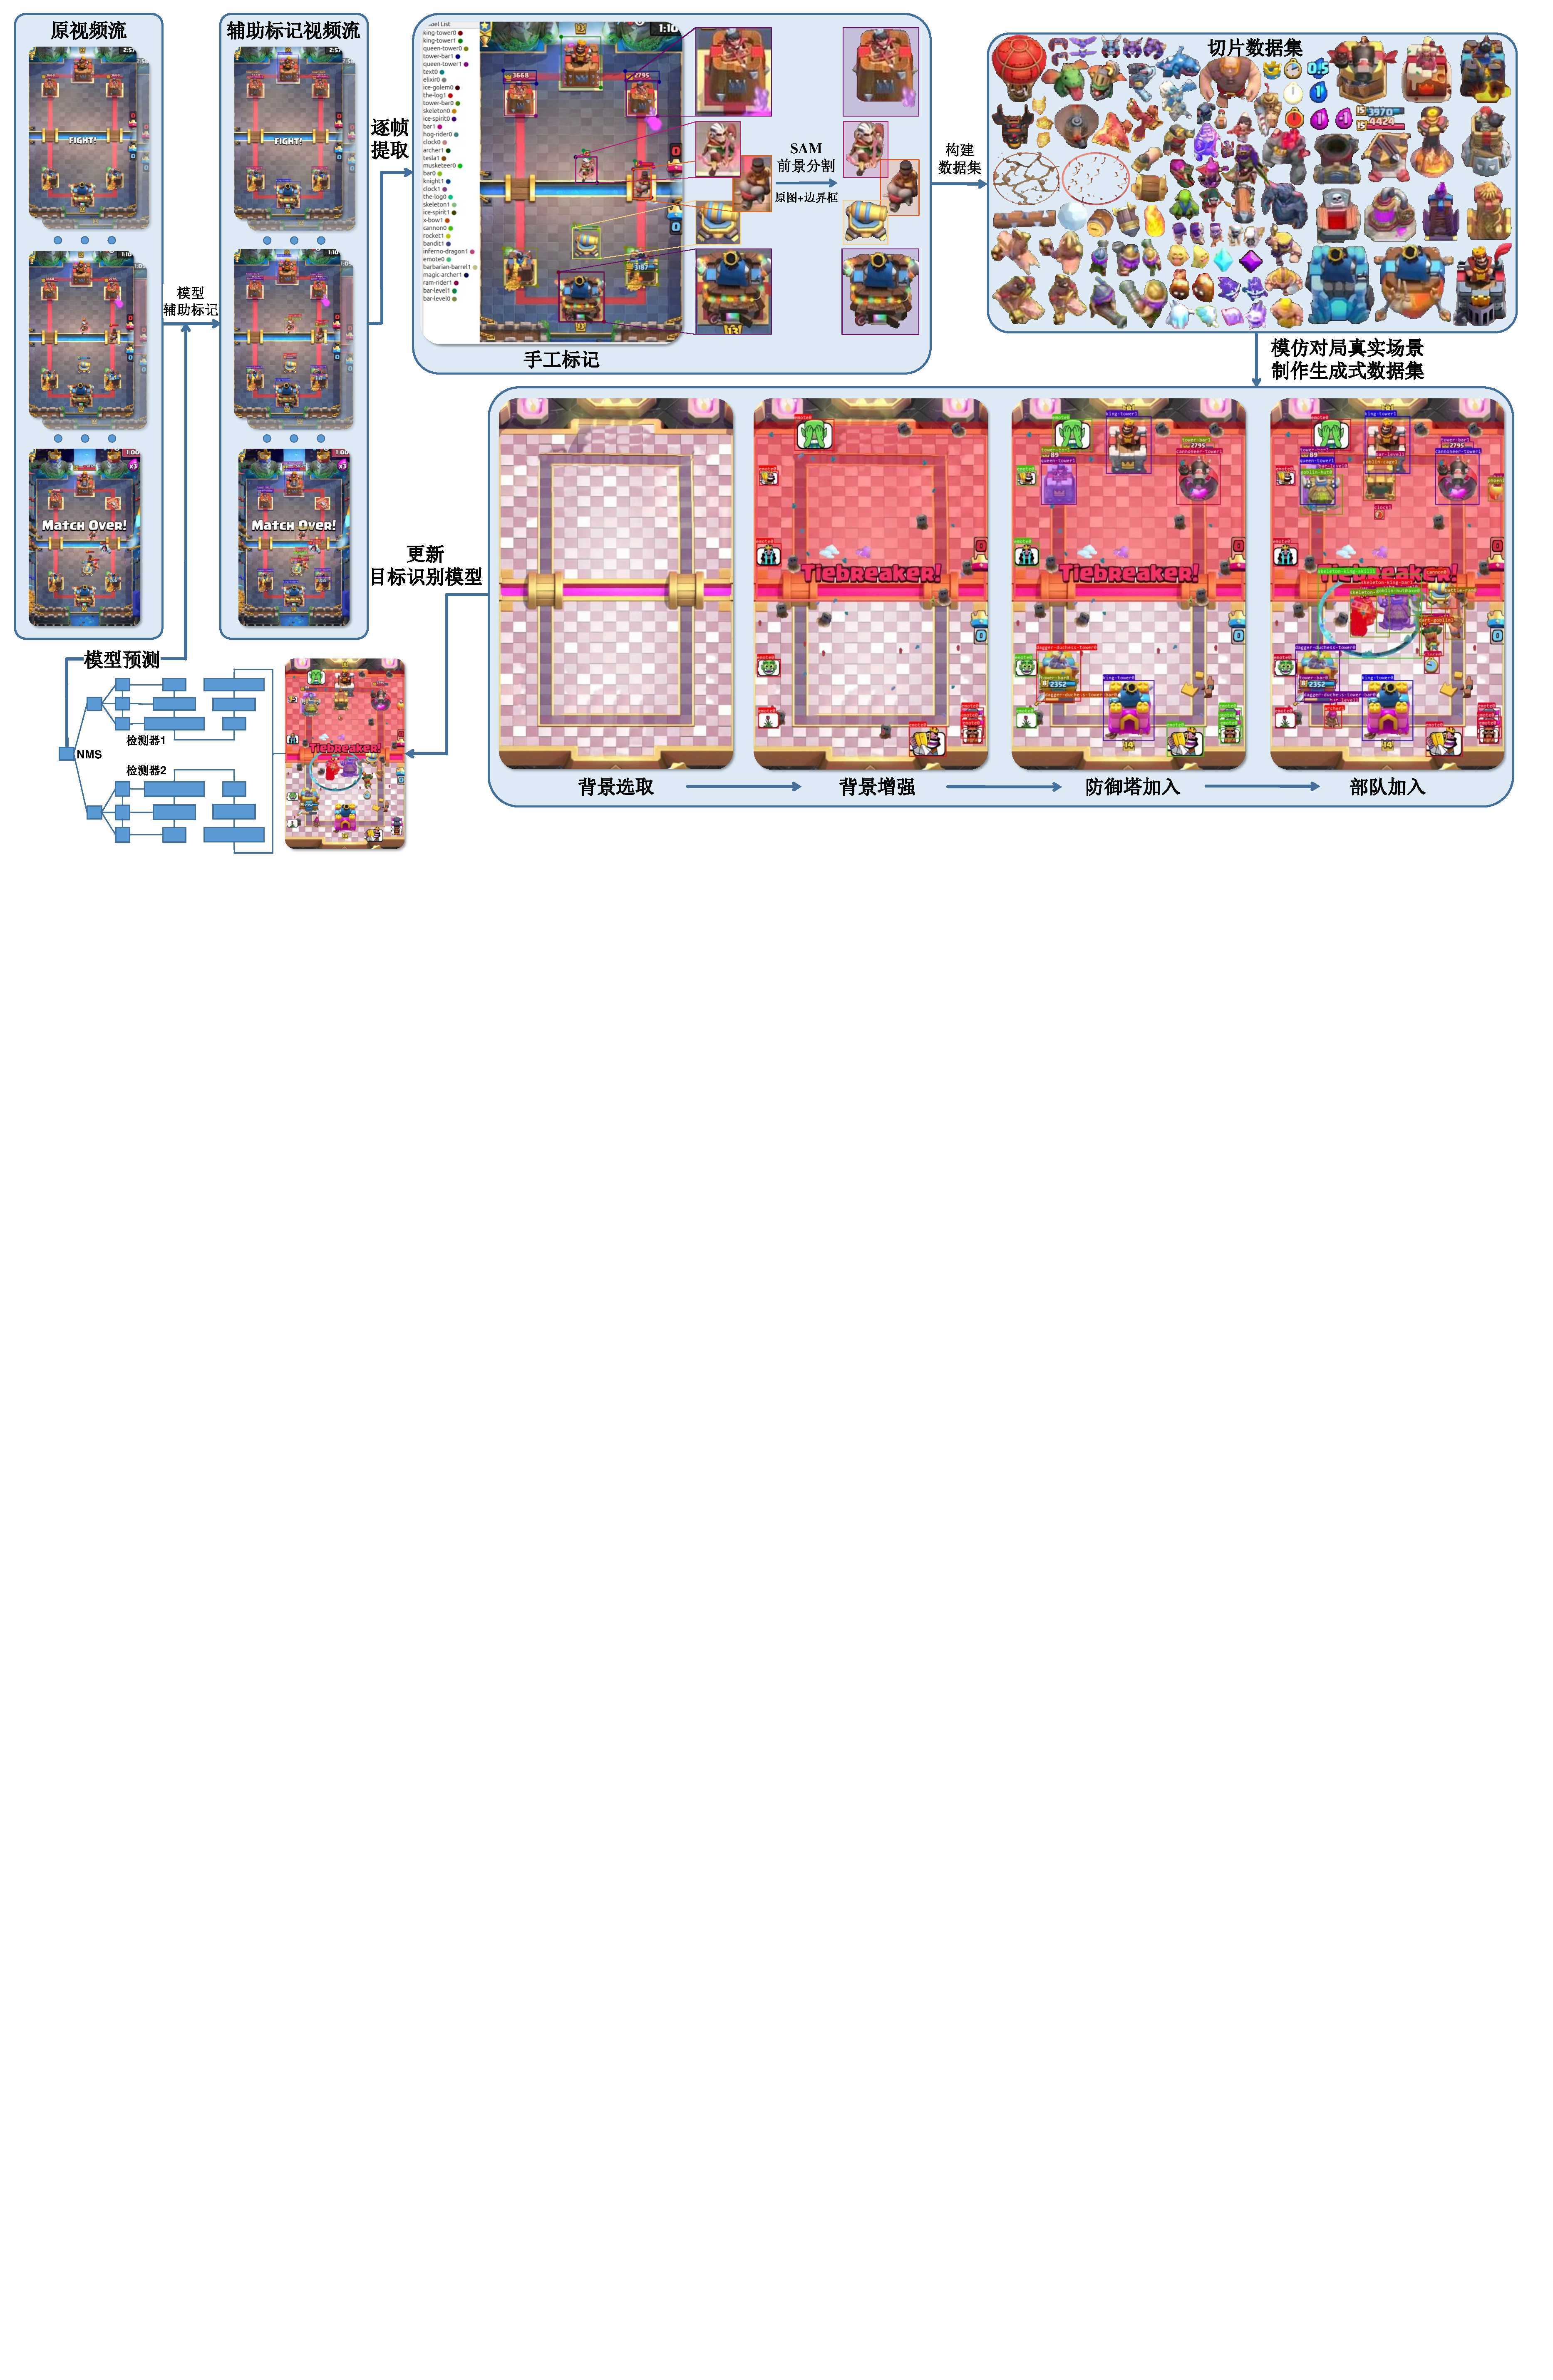
\includegraphics[width=\textwidth]{detection dataset building.pdf}
  \caption{目标识别生成式数据集制作流程}\label{fig-generation-dataset}
\end{figure}
\subsection{生成算法}
假设将每个切片作为绘制单位,第$i$个生成对象定义为$g_i = (img_i,box_i,level_i)$,
其中$img_i$为第$i$个对象对应的切片图像;
$box_i$为第$i$个对象对应的边界框,可以表示为$(x,y,w,h,c,bel)$,
其中$(x,y)$为切片中心点在整个图片中的坐标,$(w,h)$为切片宽高,$c$为当前切片类别,$bel$为当前切片的所属派别;
$level$为当前切片的所属图层等级,生成切片时按照图层从低到高依次生成切片,
图层的划分如表~\ref{tab-level}~所示。
\begin{table}[htbp]
	\renewcommand{\arraystretch}{1.2}
	\centering\wuhao
	\caption{图层等级与切片类别关系表} \label{tab-level} \vspace{2mm}
	\begin{tabularx}{\textwidth} { 
   >{\centering\arraybackslash\hsize=.6\hsize}X 
   >{\centering\arraybackslash}X }
	\toprule[1.5pt]
		图层等级 & 切片类别 \\
	\midrule[1pt]
		0 & 地面法术,地面背景部件 \\
		1 & 地面部队,防御塔 \\
		2 & 空中部队,空中法术 \\
		3 & 其余待识别部件,空中背景部件 \\
	\bottomrule[1.5pt]
	\end{tabularx}
\end{table}

绘制单位的插入流程如图~\ref{fig-generation-dataset}~中右下角部分所示,具体细节如下:
\begin{enumerate}
  \item 背景选取:从数据集中随机选取一个去除防御塔、部队及文本信息的空竞技场作为背景图片。
  \item 背景增强:加入背景板中的非目标识别部件,用于数据增强,例如:部队阵亡时的圣水,场景中随机出现的蝴蝶、花朵等。
  \item 防御塔加入:在双方的三个防御塔固定点位上随机生成完好或被摧毁的防御塔,并随机选取生成与之相关联的生命值信息。
  \item 部队加入:按照类别出现次数的反比例$\left\{\frac{1}{n_{c_i}-n_{\min}+1}\right\}_{i=1}^{|C|}$\vspace{0.5ex}
  所对应的分布进行类别随机选取,其中$n_{c_i},(c_i\in C)$表示类别$c_i$的切片之前生成的总次数,
  $n_{\min}=\min\{n_{c_i}\}_{i=1}^{|C|}$;在竞技场中按照动态概率分布(具体见附录~\ref{app-dynamic-distrib})随机选择生成点位,
  并随机选取生成与之相关的等级、生命值、圣水、时钟等信息。
\end{enumerate}

\begin{algorithm}[ht]
	\caption{生成算法伪代码\label{alg-generator}}
	\IncMargin{2em}
	\DontPrintSemicolon
	\KwIn{绘制单位序列$U=\{u_i\}$,覆盖率阈值$\alpha$,待识别类别集合$C$}
	\KwOut{image, box}
  $\text{image}\gets$空图像,$\text{box}\gets \{\}$\tcp*{初始化参数}
  $U\gets \{u_i\in U: u_i^{level}>u_j^{level}, \forall i, j \in \{1,\cdots,|U|\} \text{~且~} i < j\}$\;
  \While{True}{
    $\text{mask}\gets$空掩码,$U_{avail}\gets U$\;
    \For{$i=1,2,\cdots,|U|$}{
      \If{$\frac{u^{img}_i\cap~ \text{mask}}{u_i^{img}} > \alpha$}{
        $U_{avail}\gets U_{avail} - R(u_i)$\tcp*{删除与$u_i$相关联的单位}
      }
      $\text{mask}\gets \text{mask}\cup u_i^{img}$\;
    }
    \If{$|U_{avail}|=|U|$}{
      break\tcp*{覆盖单位筛选完成}
    }
    $U\gets U_{avail}$
  }
  $U\gets \{u_i\in U: u_i^{level}<u_j^{level}, \forall i, j \in \{1,\cdots,|U|\} \text{~且~} i < j\}$\;
  \For{$i=1,2,\cdots,|U|$}{
    $\text{img}\gets \text{img} \cup u_i^{img}$\tcp*{图像绘制}
    \If{$u_{i}^{\text{cls}}\in C$}{
      $\text{box}\gets \text{box} \cup u_i^{box}$\tcp*{边界框保存}
    }
  }
\end{algorithm}
\newpage
完成绘制单位加入后,可以按照插入顺序得到待绘制单位序列$U$,但生成的切片可能存在覆盖关系,因此需要引入最大覆盖率阈值$\alpha$,
当被覆盖单位面积超过该单位切片面积的$\alpha$倍时,对被覆盖单位进行去除,对单位完成筛选之后,
再按照图层等级的从低到高进行绘制,并将识别类别$C$中的边界框信息进行记录,用于后续识别模型训练,
具体绘制流程见算法~\ref{alg-generator}。% 通过该生成式算法得到的带标签图像如图~\ref{fig-generation}~所示。
通过调整不同的单位生成数量、切片生成类型,最大覆盖阈值$\alpha$,可以得到如图~\ref{fig-generation}~所示的生成结果。
\begin{figure}[h!]
\centering\vspace{-0.0ex}
\subfigure[单位生成数量20,小型切片类型,$\alpha=0.5$]{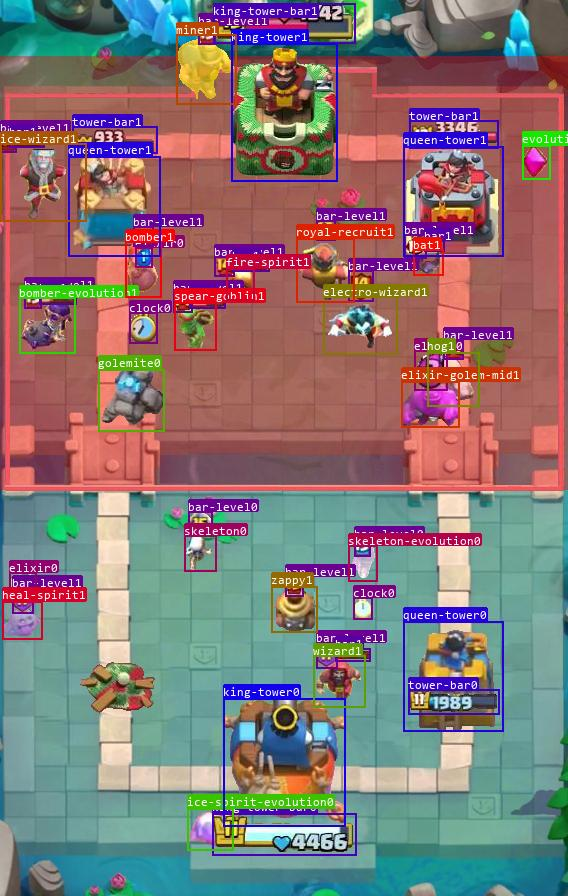
\includegraphics[width=0.32\textwidth]{generation/nu20,small,0.5.jpg}}
\subfigure[单位生成数量20,大型切片类型,$\alpha=0.5$]{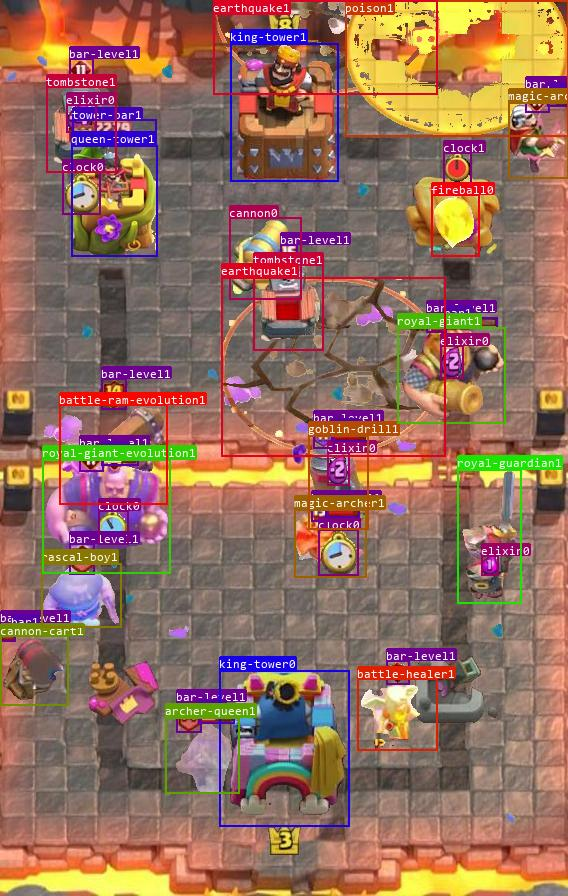
\includegraphics[width=0.32\textwidth]{generation/nu20,big,0.5.jpg}}
\subfigure[单位生成数量40,大型切片类型,$\alpha=0.8$]{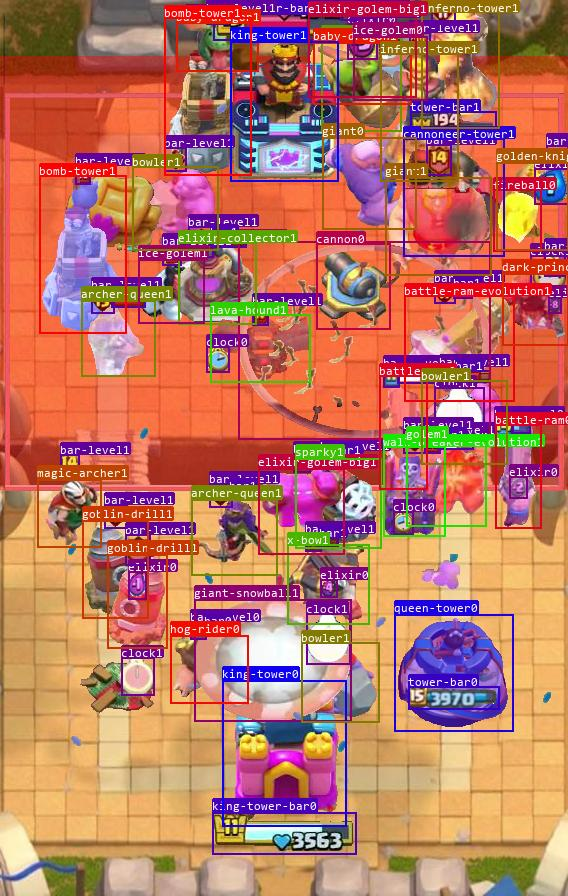
\includegraphics[width=0.32\textwidth]{generation/nu40,big,0.8.jpg}}
\setlength{\abovecaptionskip}{0ex}  % 由于minted会增大图像与标题间距需要进行缩小
\caption{生成式数据集实例}\label{fig-generation}
\end{figure}
\subsection{目标识别损失函数设计}
我们沿用Joseph Redmon等人\cite{YOLO}提出的YOLO模型损失函数。
设当前目标识别模型输出的网格步长为$s$,输入图像的大小为$W\times H$,每个网格处所需的预测框数目为$B$,
第$i$行$j$列网格预测出的第$k$个预测框记为$\left(\widehat{box}_{ijk},\hat{c}_{ijk}, \hat{p}_{c_{ijk}}, \widehat{bel}_{ijk}\right)$,
对应的目标框$\left(box_{ijk}, c_{ijk}, bel_{ijk}\right)$,\vspace{0.5ex}
则该步长下的损失函数如式 (\ref{eq-yolo-loss}) 所示。
\begin{equation}\label{eq-yolo-loss}
\begin{aligned}
\mathcal{L}_{s}(\hat{y}, y) = 
\sum_{i=1}^{H/s}\sum_{j=1}^{W/s}\sum_{k=1}^B&\ \mathbbm{1}^{noobj}_{ijk}\lambda_{noobj}\mathcal{L}_{\text{BCE}}(\hat{c}_{ijk},0)\\
&\ +\mathbbm{1}^{obj}_{ijk}\bigg[\lambda_{box}\mathcal{L}_{\text{CIOU}}\left(\widehat{\text{box}}_{ijk},\text{box}_{ijk}\right)+
\lambda_{obj}\mathcal{L}_{\text{BCE}}\left(\hat{c}_{ijk},\text{IOU}_{pred}^{true}\right)\\
&\ \qquad\qquad+\lambda_{class}\sum_{c=1}^{C}\mathcal{L}_{\text{BCE}}\bigg(\left\{\hat{p}_{ijk}\right\}_c, \text{onehot}\left(c_{ijk}\right)_c\bigg)\\
&\ \qquad\qquad+\lambda_{class}\mathcal{L}_{\text{BCE}}\left(\widehat{bel}_{ijk}, bel_{ijk}\right)\bigg]
\end{aligned}
\end{equation}
其中$\mathbbm{1}^{noobj}_{ijk}$当网格$(i,j)$下的第$k$个预测框没有对应的目标框时为$1$,反之为$0$,
相反的$\mathbbm{1}^{obj}_{ijk} = 1-\mathbbm{1}^{noobj}_{ijk}$,
$\mathcal{L}_{\text{CIOU}}$为Zheng等人\cite{CIOU}提出的Complete-IOU损失,
$\mathcal{L}_{\text{BCE}}$为二元交叉熵损失,
$\lambda_{noobj},\lambda_{box},\lambda_{obj},\lambda_{class}$
分别为无标签,边界框位置信息,置信度以及类别对应损失的加权系数。

\section{决策模型}\label{sec-decision-model}
\subsection{特征设计}
\subsubsection{状态}
模型的状态输入由2部分构成,分别为$S^{img}, \bd{s}^{card}$,其中$S^{img}\in\mathbb{R}^{18\times 32\times 15}$为单位的网格状特征输入,
对于第$i$行$j$列的特征$\bd{z}_{ij}:=(S^{img})_{ij}\in\mathbb{R}^{15}$
表示处于该位置的单位具有如下$4$种特征:$(\bd{z}_{ij})_{1:8}$为类别编码,
$(\bd{z}_{ij})_9$为从属派别编码,$(\bd{z}_{ij})_{10:12}$为生命值图像编码,$(\bd{z}_{ij})_{13:15}$为其余条状图像编码;
$\bd{s}^{card}\in\mathbb{R}^6$表示当前状态下的两个全局特征:$(\bd{s}^{card})_{1:5}$为当前手牌信息,
$(\bd{s}^{card})_6$为当前总圣水量。

\subsubsection{动作}
模型的动作输入由2个部分构成:$\bd{a}^{pos}, a^{select}$,其中$\bd{a}^{pos}\in\mathbb{R}^2$表示动作执行的部署坐标,
$a^{select}$表示动作执行的手牌编号。

\subsubsection{奖励}\label{sec-reward}
奖励设计如下,设$h_{i}^{\text{bel}}, (i\in\{0,1,2\},\text{bel}\in\{0,1\})$为防御塔生命值,
当$i=1,2$时表示左右两个副塔生命值,$i=0$表示主塔生命值,$\text{bel}=0,1$分别表示我方和敌方建筑,
$\Delta h_{i}^{\text{bel}}$表示前一帧与当前帧生命值的差值,$H_{i}^{\text{bel}}$表示对应防御塔的总生命值,分别定义如下四种奖励函数:

1. 防御塔生命值奖励
\begin{equation}
  r_{tower} = \sum_{\text{bel}=0}^1\sum_{i=0}^2(-1)^{\text{bel}+1}\frac{\Delta h_{i}^{\text{bel}}}{H_{i}^{\text{bel}}}
\end{equation}

2. 防御塔摧毁奖励$r_{distory}$:当敌我副塔被摧毁时给予$(-1)^{\text{bel}+1}$奖励,敌我主塔被摧毁时给予前者的$3$倍奖励。

3. 主塔激活奖励$r_{activate}$:当副塔均存活的条件下,主塔第一次失去生命值时,给予$(-1)^{\text{bel}}~0.1$奖励。

4. 圣水溢出惩罚$r_{elixir}$:当总圣水持续保持溢出状态时,每间隔$1$秒产生一次$0.05$的惩罚。

综合上述奖励,得到总奖励
\begin{equation}\label{eq-reward}
  r = r_{tower} + r_{destory} + r_{activate} + r_{elixir}
\end{equation}
\subsection{离线强化学习}\label{sec-model-design}
首先对强化学习中概念进行介绍,
考虑无限长带折扣Markov决策过程(Markov Decision Process, MDP),定义为$(\mathcal{S},\mathcal{A},p,r,\gamma)$,
其中$\mathcal{S}$为状态空间,$\mathcal{A}$为动作空间,
$p:\mathcal{S}\times \mathcal{A}\times \mathcal{S}\to \mathbb{R}$为状态转移方程,
$r:\mathcal{S}\times\mathcal{A}\to \mathbb{R}$为奖励函数,$\gamma\in(0,1)$为折扣系数。
令$\pi$表示决策函数$\pi: \mathcal{S}\times \mathcal{A}\to [0,1]$,令$R(\pi)$表示其期望所获得的总奖励(回报):
\begin{equation}
  R(\pi) = \mathbb{E}_{S_1,A_1,S_2,A_2\cdots}\left[\sum_{t=0}^{\infty}r(S_t,A_t)\right],\quad
  \text{~其中~}A_t\sim\pi(\cdot|S_t),S_{t+1}\sim p(\cdot|s_t,a_t)
\end{equation}
强化学习的目标通常是找到最优策略$\pi^* := \argmax_{\pi}R(\pi)$,
在线强化学习算法往往通过策略迭代和价值函数估计方法实现策略的更新,
而本文中所使用的离线强化学习算法不再基于值估计方法,而是更加类似于模仿学习的方法。

Chen等人\cite{DT}的Decision Transformer(DT)是一种将强化学习问题是为序列建模问题的方法,使用了深度学习中的Transformer架构,
对于离线数据集中的一段长度为$T$的交互轨迹(Trajectory)
\begin{equation}
  \rho = (s_1,a_1,r_1,s_2,a_2,r_2,\cdots,s_T,a_T,r_T,s_{T+1})
\end{equation}
其中$s_{T+1}$为终止状态,则$\rho$可以视为建模为序列
\begin{equation}\label{eq-sequence}
  R_0,s_1,a_1,R_1,s_2,\cdots,a_{T-1},R_{T-1},s_{T},a_{T}
\end{equation}
其中$R_i=\sum_{t=i}^Tr_{t+1}, (i=0,\cdots,T-1)$为目标回报(Return-to-Go)。

DT模型中序列编码模型使用的是Radford等人\cite{GPT}的GPT模型,即仅含有编码器的因果注意力机制。
因果注意力(Causal Attention)为(每个特征$i$只能看到$j\leqslant i$的特征)
\begin{equation}\label{eq-attn}
\begin{aligned}
  Z = \text{softmax}\left(\frac{\left(QK^T\right)\odot M}{\sqrt{d_k}}\right)V
\end{aligned}
\end{equation}
其中$M$被成为掩码矩阵,为$N$阶下三角阵,$Q,K,V$分别表示输入序列$X$对应生成的询问键(Query),查询键(Key)和价值键(Value),
询问键与查询键具有相同的特征维度$d_k$。
当式 (\ref{eq-attn}) 中$M$为全$1$矩阵时,$Z$定义为交叉注意力(Cross Attention)。

\begin{figure}[htbp]
  \centering\vspace{-2ex}
  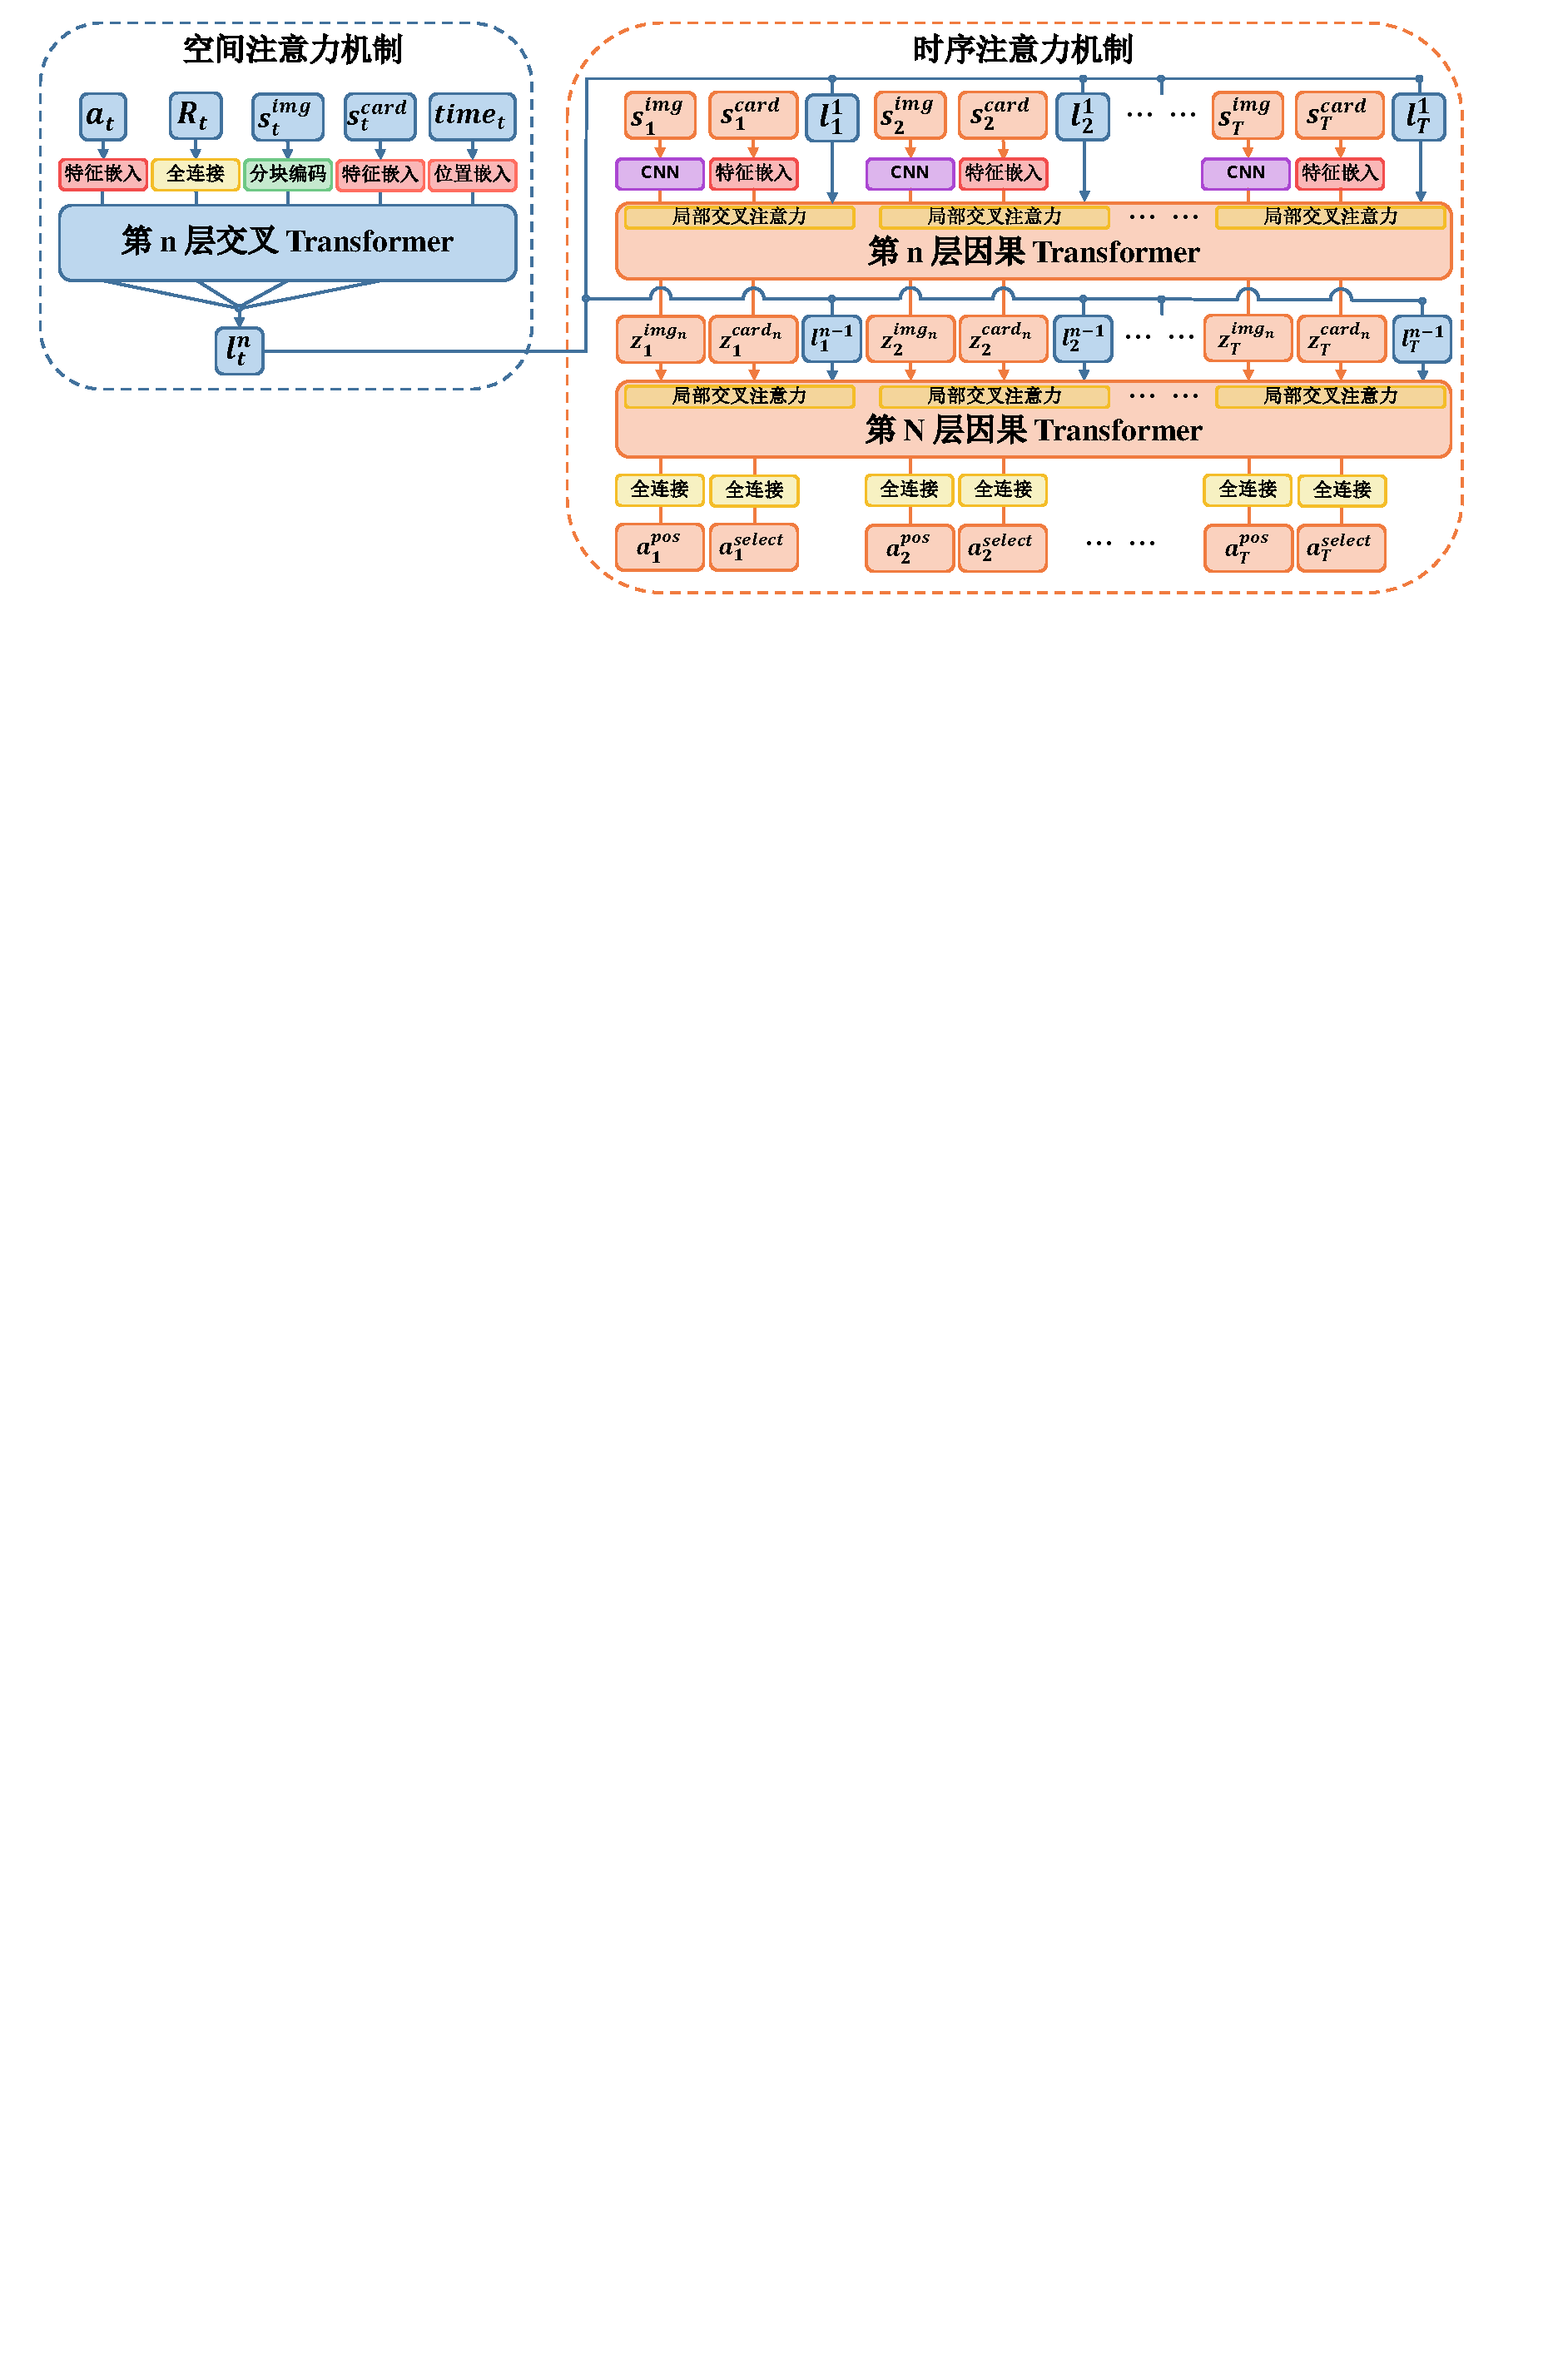
\includegraphics[width=\textwidth]{policy_model.pdf}
  \caption{决策模型架构,左侧的空间注意力机制用于编码同一时刻下的特征信息,
  右侧的时序注意力机制用于关联上下帧信息,做出动作预测}
  \label{fig-model}
\end{figure}

我们设计的模型如图~\ref{fig-model}~所示,
基于Shang等人的\cite{StARformer}StARformer的ViT+DT的架构,
模型输入为轨迹序列$(a_t, R_t, s_t)_{t=1}^T$,
输出为动作预测序列$(a_t^{pos},a_t^{select})_{t=1}^T$。左侧交叉注意力机制对
局部信息$(a_t,R_t,s_t)$按空间维度进行编码,并使用ViT中分块思路将图像$s_t^{img}$转化为序列;
右侧为因果注意力机制对全局信息$(s^{img}_t,s^{card}_t)$按时序维度进行编码,
并在每层序列输入中引入对应的局部编码信息$l_t^{n}$。
由于需要使同一时刻下的信息可以相互产生注意力关系,所以需要引入局部交叉注意力,
具体实现方法是将式 (\ref{eq-attn}) 中的掩码矩阵 $M$ 定义为 $M_{3}$,其中
\begin{equation}
  (M_{L_0})_{ij} = \begin{cases}
    1, &\quad i=kL_0-l,j\leqslant kL_0\\
    0, &\quad \text{否则}
  \end{cases},\quad k\in\{1,\cdots,L\}, l\in\{0,\cdots,L_0-1\}
\end{equation}

设输入的轨迹的长度为$L$,$\mathbbm{H}$表示占位符,我们设计了三种模型架构:
\begin{itemize}
  \item \textbf{StARformer-3L} 模型输入序列长度为$3L$,第$n$层Cause Attention Transformer输出的时序序列记为
  $\{z_t^{img_n},z_t^{card_n},l_{t}^{n-1}\}_{t=1}^{L}$,局部注意力中掩码矩阵为$M_3$,
  输出与$(a_t^{pos},a_t^{select},\mathbbm{H})_{t=1}^T$对应。
  \item \textbf{StARformer-2L} 模型输入序列长度为$2L$,第$n$层Cause Attention Transformer输出的时序序列记为
  $\{z_t,l_{t}^{n-1}\}_{t=1}^{L}$,局部注意力中掩码矩阵为$M_2$,
  输出与$(\left[a_t^{pos},a_t^{select}\right],\mathbbm{H})_{t=1}^T$对应。
  \item \textbf{DT-4L} 模型输入长度为$4L$,仅包含时序注意力机制中的Cause Attention Transformer,
  第$n$层Transformer的输出的时序序列为$\{a_{t-1},R_{t-1},s_{t}^{img_n}, s_{t}^{card_n}\}_{t=1}^{L}$,
  输出与$(\mathbbm{H},\mathbbm{H},a_{t}^{pos},a_{t}^{select})_{t=1}^T$对应。
\end{itemize}

\subsection{预测目标设计与重采样}\label{sec-target-and-resample}
由于本任务中动作执行极为离散,总帧数中仅有$4\%$为执行动作帧,其余帧均不执行动作,
如果直接逐帧预测动作会产生非常严重的长尾问题,
导致模型最终基本不执行动作(表~\ref{table-model-eval}~中离散预测的动作数远低于连续动作预测数),
因此需要将预测目标从离散转化为连续,解决方法是引入延迟动作预测:
对于第$i$帧,需找到其后(包含自身)最近的动作帧$j$,令最大间隔帧数阈值为$T_{delay}$,
则每个非动作帧的预测的延迟动作为$a^{delay}_{i} = \min\{j-i, T_{delay}\}$。

对离线数据集进行采样时,为避免长尾问题导致模型偏移,本文还设置了重采样频次,
设数据集总帧数为$N$,动作帧数为$N_{action}$,则动作帧占比为$r_a:=N_{action} / N$,
对于第$i$个动作帧位于数据集中的第$t_i$帧,则轨迹的结束帧$j\in\{t_{i},\cdots,t_{i+1}-1\}$对应的重采样频次为
\begin{equation}\label{eq-resample-freq}
  s_j = \max\left\{\frac{1}{1-r_a}, \frac{1}{r_a(j-t_i+1)}\right\},\quad (t_i\leqslant j\leqslant t_{i+1})
\end{equation}
则训练轨迹中结束帧的采样分布为$\left\{\frac{s_j}{\sum_{j=1}^{N}s_j}\right\}_{j=1}^N$,
图~\ref{fig-resample-and-delay}~中展示了离线数据集一段轨迹所对应的重采样频次与动作预测值。
\begin{figure}[htbp]
  \centering
  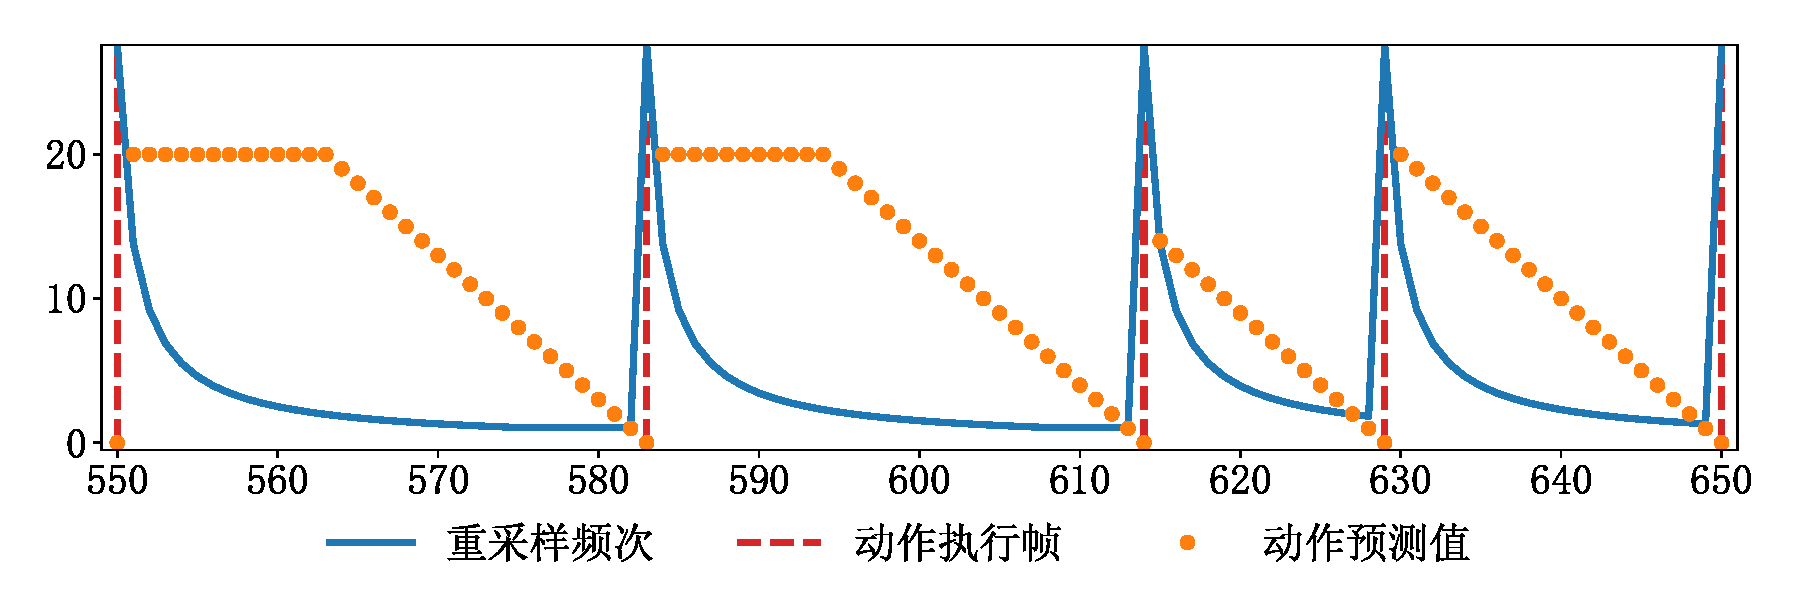
\includegraphics[width=\textwidth]{resample_and_delay.pdf}
  \caption{从离线数据集中截取的一段数据,总共包含5个动作帧,最大间隔帧数阈值$T_{delay} = 20$,}\label{fig-resample-and-delay}
\end{figure}

\section{数据分析及实验结果}
本章对前3章内容的实验结果进行总结,分别包含第 \ref{sec-generation-dataset} 章的生成式数据集分析统计和目标识别模型对比实验,
以及 \ref{sec-decision-model} 的决策模型对比实验。

\subsection{生成式数据集分析}{}\label{sec-exp-data}
数据集总共分为两部分\footnote{上述数据集统计信息截止于2024年5月6日,全部图像数据集均已开源:
\url{https://github.com/wty-yy/Clash-Royale-Detection-Dataset}}:
\begin{enumerate}
  \item 生成式数据集切片:总计$154$个类别,待识别类别$150$个,总共包含$4654$个切片,
  在全部待识别类别的切片图像中,切片大小分布如图~\ref{fig-segment}~所示。
  \item 目标识别验证集:总计$6939$张人工标记的目标识别图像,包含$116878$个目标框,平均每张图片包含17个目标框,该数据集均为真实对局视频流逐帧标记得到,
  而模型训练所使用的完全是生成式数据集,所以该数据集可以做验证集使用。
\end{enumerate}

\begin{figure}[htbp]
  \centering
  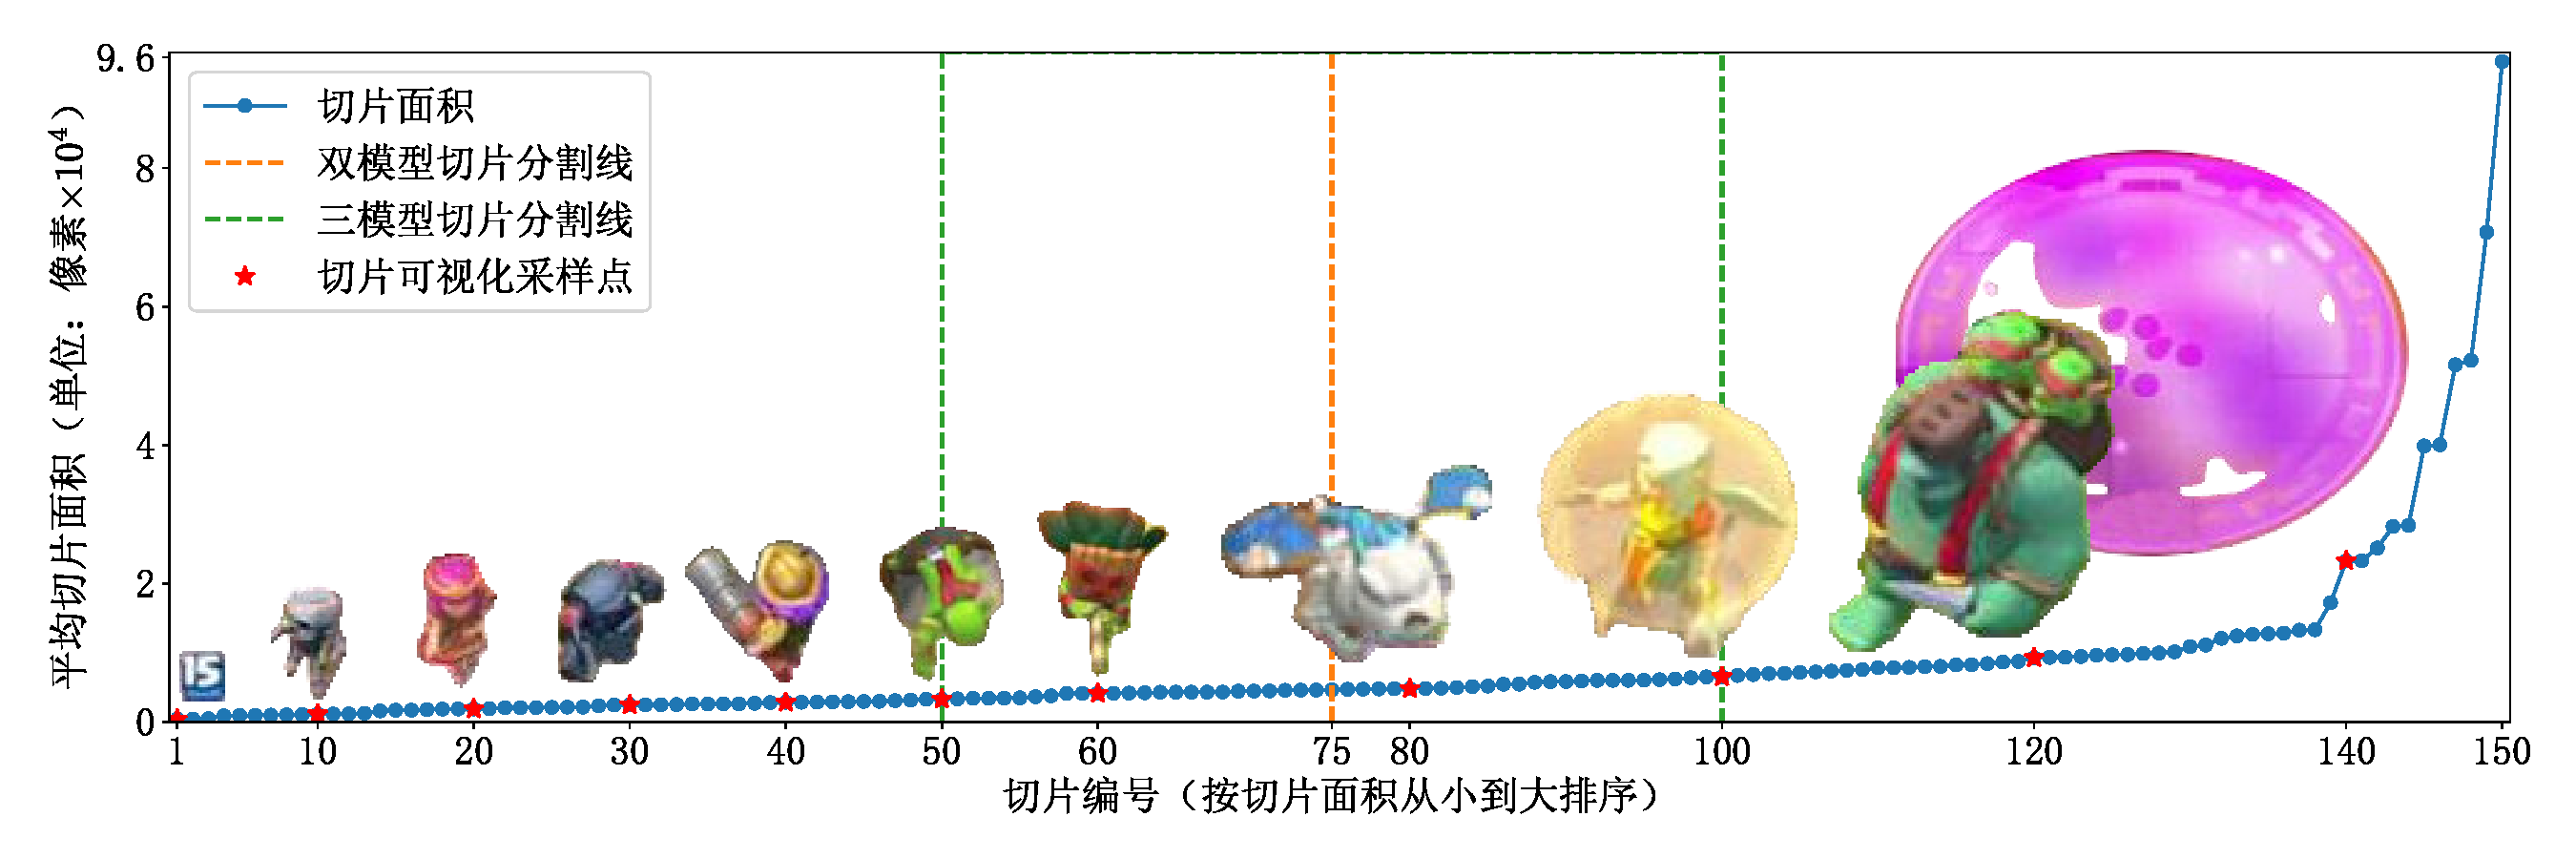
\includegraphics[width=\textwidth]{segment_size.pdf}
  \caption{将切片数据集全部切片按平均面积从小到大排序并编号,
  从中随机采样出部分切片进行可视化。
  分别以全体切片面积的二等分和三等分点,作为双模型和三模型的识别类别分割线。
  }
  \label{fig-segment}
\end{figure}

\subsection{目标识别模型}{}\label{sec-exp-detect}
目标识别模型使用了自己实现的YOLOv5\footnote{复现YOLOv5代码:\url{https://github.com/wty-yy/KataCV/tree/master/katacv/yolov5}}
和重构后的YOLOv8的模型\footnote{YOLOv8重构内容:\url{https://github.com/wty-yy/KataCR/blob/master/asserts/yolov8_modify.md}},
每个训练集大小设置为$20000$,至多训练$80$个epoch收敛。
数据增强使用了:HSV增强,图像旋转,横纵向随机平移,图像缩放,图像左右反转,具体参数见附录表~\ref{table-app-aug}~。

实验结果\footnote{YOLOv5全部训练曲线:\url{https://wandb.ai/wty-yy/ClashRoyale},YOLOv8全部训练曲线:\url{https://wandb.ai/wty-yy/YOLOv8}}如表~\ref{tabel-yolo}~所示,表中具体内容解释如下:

1. 模型名称:编号后的字母表示模型大小,l,x分别对应大与特大型模型,
YOLOv8-l$\times n$表示使用$n$个YOLOv8-l模型,每个子模型分别识别图~\ref{fig-segment}~中分割线所划分区域中的切片类型,
最后将识别的预测框通过非最大值抑制(Non-Maximum Suppression,NMS)进行筛选,NMS过程中IOU阈值设定为0.6。

2. 评测指标:表中mAP评测指标表示COCO mAP指标\upcite{COCO},即在10种不同IOU阈值下计算PR曲线下面积求平均得到,
AP50、P50、R50和mAP(S)分别表示在判断正例的IOU阈值为$50\%$下的mAP、平均精度、平均召回率和小目标的mAP。

3. 验证速度:模型预测时Batch大小设置为$1$,FPS为模型在GeForce RTX 4090下测试的验证速度,验证测试时置信度设置为$0.001$。
当对视频流数据进行预测时,将置信度改为$0.1$,并使用ByteTrack\upcite{ByteTrack}算法在目标追踪计算过程中对边界框进行筛选,
FPS(T)是在GeForce RTX 4060 Laptop下带有目标追踪的识别速度。

从实验结果可以看出,YOLOv8-l的双识别器对小目标的识别能力与三识别器效果基本一致,并远高出非组合式的识别器,
其原因可能在于$150$个预测类别大小远超模型的识别能力范围,
最大目标与最小目标的边界框大小差距甚远,又由于YOLOv8是无锚框识别头,
由于大目标易于识别,可能导致预测的目标框均偏大,所以多个识别器降低平均类别数能够有效对小目标进行识别。

\begin{table}[!h]
	\renewcommand{\arraystretch}{1.2}
	\centering\wuhao
	\caption{YOLO模型对比测试结果} \label{tabel-yolo} \vspace{2mm}
	\begin{tabularx}{\textwidth} { 
   >{\centering\arraybackslash}X 
   >{\centering\arraybackslash\hsize=.3\hsize}X
   >{\centering\arraybackslash\hsize=.2\hsize}X
   >{\centering\arraybackslash\hsize=.2\hsize}X
   >{\centering\arraybackslash\hsize=.3\hsize}X
   >{\centering\arraybackslash\hsize=.4\hsize}X
   >{\centering\arraybackslash\hsize=.3\hsize}X
   >{\centering\arraybackslash\hsize=.4\hsize}X
   >{\centering\arraybackslash\hsize=.9\hsize}X 
   >{\centering\arraybackslash\hsize=.7\hsize}X
  }
	% \toprule[1.5pt]
  \hline
  模型名称&AP50&P50&R50&mAP&mAP(S)&FPS&FPS(T)&检测器类别数&数据增强\\
  \hline
	% \midrule[1pt]
  YOLOv5-l&66.2&84.4&63.8&53.2&NA&59&NA&151&\\
  YOLOv8-x&83.1&\pmb{93.9}&68.3&67.7&39.8&68&31&160&\\
  YOLOv8-x&\pmb{85.3}&90.7&80.4&66.8&35.9&68&31&160&\checkmark\\
  YOLOv8-l~$\times 2$&84.3&89.5&79.8&67.4&43.9&34&18&85&\checkmark\\
  YOLOv8-l~$\times 3$&85.2&89.7&\pmb{80.9}&\pmb{68.8}&\pmb{48.3}&23&10&65&\checkmark\\
  \hline
	% \bottomrule[1.5pt]
	\end{tabularx}
\end{table}

\subsection{决策模型}\label{sec-decision-model}
我们手动构建了玩家与与游戏内置的$8000$分AI对局$105$回合的专家数据
\footnote{专家数据集:\url{https://github.com/wty-yy/Clash-Royale-Replay-Dataset}},
固定双方使用的卡组,
数据集总计$113981$帧,动作帧占比$4.01\%$,重采样频次比率为$\frac{\text{动作帧}}{\text{非动作帧}}=24.92:1.04$,
平均动作延迟大小为$21.26$,最大间隔帧数阈值为$T_{delay}=20$(重采样细节见~\ref{sec-target})。
模型损失函数分为三个部分,由于均为离散动作,所以损失函数均使用目标动作均使用交叉熵损失,总损失函数如下
\begin{equation}
  \mathcal{L} =
  \sum_{\substack{i=1\\}}^N\mathbb{I}_{a_i^{delay} < T_{delay}}\left[\mathcal{L}_{\text{CE}}(\hat{\bd{a}}_i^{pos}, \bd{a}_i^{pos})+
  \mathcal{L}_{\text{CE}}(\hat{a}_i^{select}, a_i^{select}) + 
  \mathcal{L}_{\text{CE}}(\hat{a}_i^{delay}, a_i^{delay})\right]
\end{equation}
其中$T_{delay},\bd{a}_i^{pos},a_i^{select},a_i^{delay}$分别为最大间隔帧数阈值、目标动作的部署坐标、手牌编号以及部署延迟,
注意每条轨迹下只考虑$a_i^{delay} < T_{delay}$对应的梯度。

本文分别测试了下述模型参数:
\begin{itemize}
  \item 不同的模型架构见~\ref{sec-model-design}~,分别测试了StARformer和DT架构。
  \item 模型输入的轨迹步长记为$L$,测试了$L=30,50,100$的情况。
  \item 不同的预测目标(离散与连续预测见~\ref{sec-target-and-resample}~)。
  \item 不同的手牌预测范围,默认预测当前手牌编号,也尝试了对当前牌库中全部手牌进行预测。
\end{itemize}

本文使用了如下数据增强方式对模型进行训练:
\begin{itemize}
  \item 重采样:对稀疏的动作帧按比例进行进行重采样,加快模型收敛,缓解离线数据集的长尾问题。
  \item 随机手牌重组:对当前输入轨迹中的全部手牌按照随机排列进行打乱,当预测全部手牌编号时,将动作对应的手牌也进行相应变换。
\end{itemize}

全部模型训练曲线均进行了上传\footnote{决策模型训练曲线:\url{https://wandb.ai/wty-yy/ClashRoyale\%20Policy}},
模型实时对局的验证结果总结于表~\ref{table-model-eval}~中,在实时对局的实现中包含以下细节:
\begin{itemize}
  \item 动作执行:对于连续动作预测模型中,由于感知识别中存在延迟,当预测动作延迟在$8$帧以内就会立刻执行动作,
  并且为了避免总圣水溢出导致的惩罚奖励,每当总圣水达到$10$时就直接下出当前预测的卡牌。
  \item 无效动作跳过:若模型预测出的卡牌所需圣水超出了当前总圣水量或当前动作执行的卡牌位为空。
\end{itemize}

\begin{table}[!h]
	\renewcommand{\arraystretch}{1.2}
	\centering\small
  %\wuhao
	\caption{决策模型对比}\label{table-model-eval}\vspace{2mm}
	\begin{tabularx}{\textwidth} { 
   >{\centering\arraybackslash\hsize=1.4\hsize}X 
   >{\centering\arraybackslash\hsize=0.6\hsize}X 
   >{\centering\arraybackslash}X 
   >{\centering\arraybackslash}X
   >{\centering\arraybackslash}X
   >{\centering\arraybackslash}X 
   >{\centering\arraybackslash}X 
   >{\centering\arraybackslash\hsize=.5\hsize}X
   }
	\toprule[1.5pt]
	模型框架&步长$L$&训练回合&总奖励&对局时长/秒&动作数&胜率\\
	\midrule[1pt]
  DT-4L&$50$&$8$&$-5.7\pm 2.5$&$148.9\pm 33.6$&$128.7\pm 37.7$&$5\%$\\
  StARformer-2L&$30$&$3$&$-6.0\pm 2.3$&$135.0\pm 35.1$&$141.8\pm 57.9$&$5\%$\\
  StARformer-2L&$50$&$8$&$-6.2\pm 2.2$&$131.9\pm 44.3$&$195.3\pm 69.8$&$5\%$\\
  StARformer-2L&$100$&$1$&$-4.9\pm 2.8$&$150.2\pm 35.6$&$187.6\pm 48.2$&$0\%$\\
  StARformer-3L&$30$&$4$&$-5.1\pm 3.7$&$147.2\pm 37.4$&$190.8\pm 52.7$&\pmb{$10\%$}\\
  StARformer-3L&$50$&$3$&\pmb{$-4.7\pm 3.1$}&\pmb{$158.9\pm 27.7$}&\pmb{$207.8\pm 48.2$}&$5\%$\\
  StARformer-3L&$100$&$5$&$-6.1\pm 2.2$&$125.9\pm 37.8$&$144.6\pm 42.9$&$5\%$\\
  \makecell[c]{StARformer-3L\\[-1ex](全卡牌预测)}&$50$&$2$&$-5.6\pm 2.1$&$150.2\pm 38.6$&$195.3\pm 69.8$&$0\%$\\
  \makecell[c]{StARformer-2L\\[-1ex](离散动作预测)}&$50$&$1$&$-7.5\pm 0.8$&$123.1\pm 39.2$&$21.9\pm 9.4$&$0\%$\\
	\bottomrule[1.5pt]
	\end{tabularx}
\end{table}

表~\ref{table-model-eval}~中记录了为每个模型的前10次训练结果中,与环境交互20个回合得到的最高平均奖励,
从中可以看出,将离散预测改为连续预测提高了$37\%$的性能、StARformer架构从2L修改为3L的改动提高了$24\%$的模型性能。
表中每列的含义分别为:
\begin{itemize}
  \item 步长$L$:为模型架构设计~\ref{sec-model-design}~中的输入轨迹长度。
  \item 训练回合:前10个训练结果中,获得最高奖励所对应的回合数。
  \item 总奖励:按奖励公式~(\ref{eq-reward})~进行累计得到的总奖励。
  \item 对局时长:统计每次对局的时长。
  \item 动作数:统计每局智能体成功执行的动作数目。
  \item 胜率:按照~\ref{win-condition}~中介绍的游戏目标,判定智能体的获胜概率。
\end{itemize}


本文使用的验证环境:手机系统为鸿蒙、电脑系统为Ubuntu24.04 LTS、CPU: R9 7940H、GPU: RTX GeForce 4060 Laptop,
平均决策用时120ms,感知融合用时240ms。

图~\ref{fig-model-eval}~中展示了每种模型前10个训练结果的验证曲线。

\begin{figure}[h!]
  \centering
  \subfigure[不同模型结构]{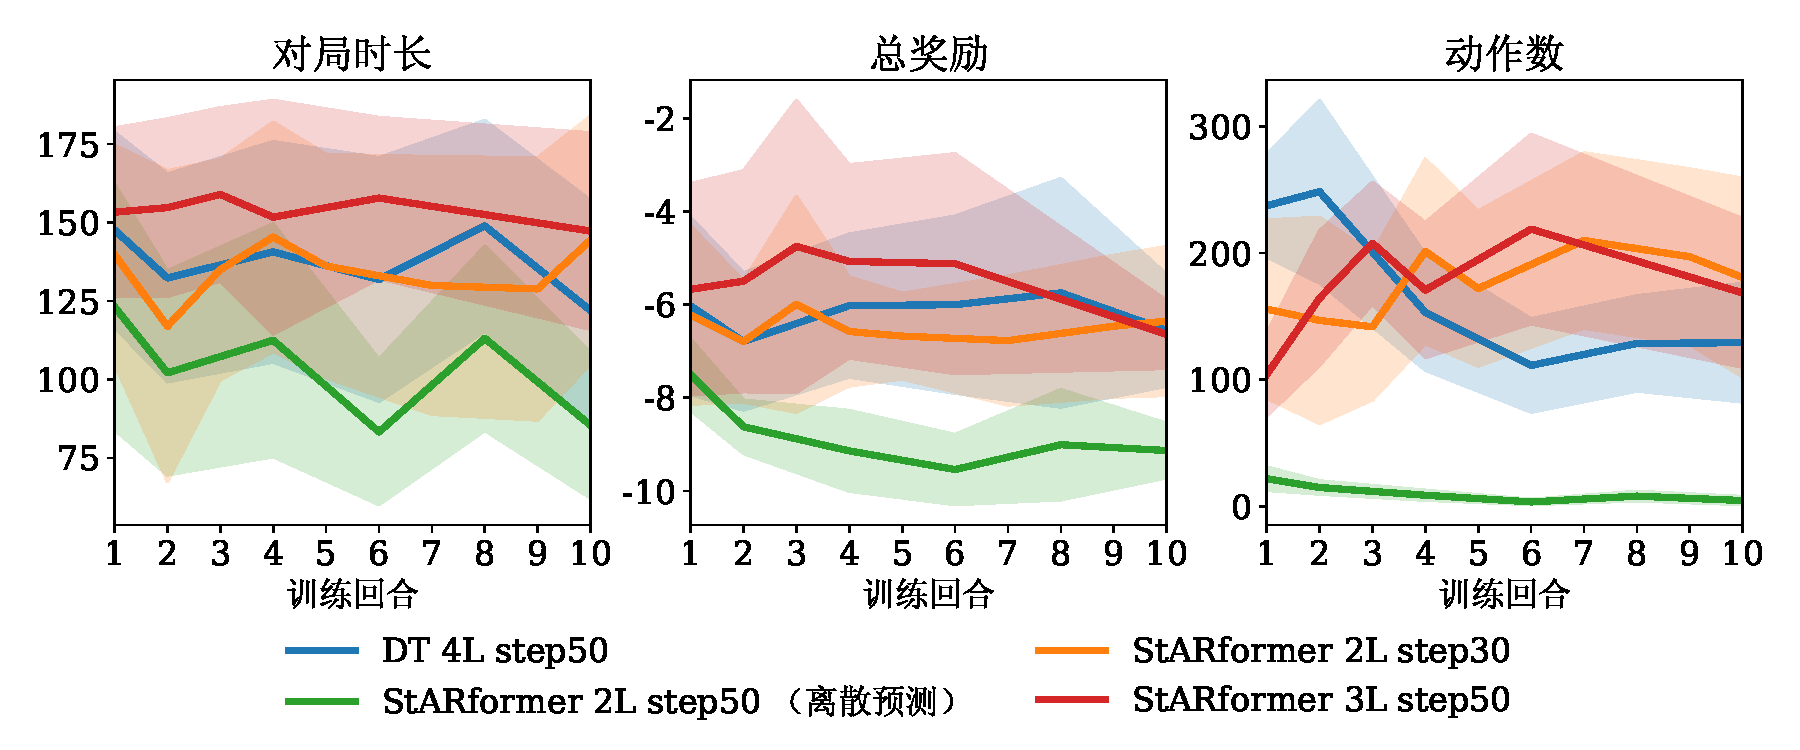
\includegraphics[width=\textwidth]{diff_model.pdf}}
  \subfigure[StARformer-3L采取不同轨迹长度]{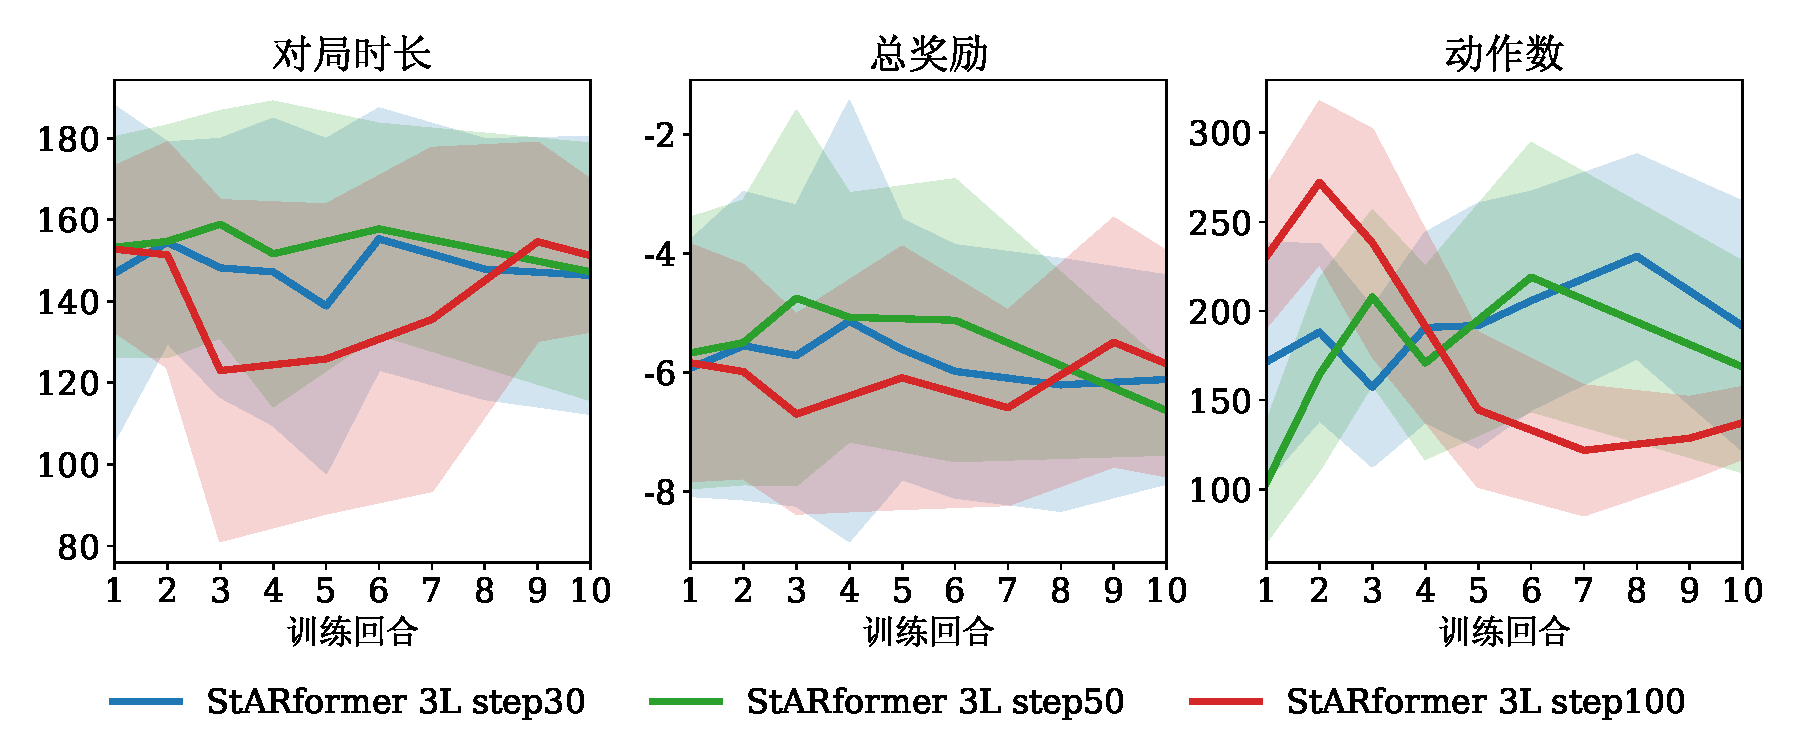
\includegraphics[width=\textwidth]{diff_3L_nstep.pdf}}
  \setlength{\abovecaptionskip}{0ex}  % 由于minted会增大图像与标题间距需要进行缩小
  \caption{模型验证曲线:展示了前10个训练结果,每回合模型在真实对局中的对局时间时长、总奖励和执行动作数,
  每次进行20次对局,实线为均值、虚影为标准差。}\label{fig-model-eval}
\end{figure}

\section{总结}

本文基于游戏皇室战争(Clash Royale),首次提出了一种基于非嵌入式的离线强化学习训练策略。
结合目标识别和光学文本识别的前沿算法,成功实现了智能体在移动设备上进行实时对局,并且战胜了游戏中的内置AI。

我们为非嵌入式强化学习在移动设备上的应用提供了新的思路。未来的工作可以从算法改进上进行拓展,
当前在固定卡组下进行训练,仍然无法$100\%$战胜游戏中的内置AI,因此远无法达到人类平均水平,
而且制作离线强化学习数据集需要花费大量的人力,
若要进一步提升智能体能力,应该需要采用在线强化学习算法,
与此同时需要使用更加高效的感知融合算法和决策模型架构,才有可能进一步提高智能体的实时决策能力和对局胜率。

本文的全部代码均已开源\footnote{全部代码:\url{https://github.com/wty-yy/katacr}},
智能体对局获胜的视频已上传\footnote{对局视频:\url{https://www.bilibili.com/video/BV1xn4y1R7GQ}},
期望能够为相关领域的研究者提供有价值的参考和借鉴。
\section{致谢}

%%% 致谢 %%%

%======================================= Reference =======================================
%%% 参考文献 %%%

\bibliographystyle{bib/xjtuthesis-numerical}
\bibliography{bib/mybib}
% \begin{thebibliography}{8}
% \bibitem{AlphaGo} 1
% \bibitem{AlphaStar} 1
% \bibitem{AlphaZero} 1
% \bibitem{OpenAIFive} 1
% \bibitem{PPO} 1
% \bibitem{DQN} 1
% \bibitem{DT} 1
% \bibitem{StARformer} 1
% \end{thebibliography}

\end{document} 
